\documentclass{article}  % //TODO find why latex gives errors for report and using textsc!
\usepackage{fancyhdr}
\usepackage{graphicx}
\usepackage{amsmath}
\usepackage{mhchem}
\usepackage{amssymb}
\usepackage[margin=1in]{geometry}

\graphicspath{{./images/}}

\title{UW CHEM 152 Notes}
\author{Anthony Le}

\newtheorem{exmp}{Example}
\newtheorem{exrc}{Excersize}
\newtheorem{proof}{Statement}
\newtheorem{defn}{Definition}


\begin{document}

\pagestyle{fancy}
\fancyhead{}
\fancyhead[R]{UW CHEM 152}
\fancyhead[L]{Anthony Le}

\begin{center}
    \LARGE{\textbf{CHEM 152 ALEKs Scratch Work}}
\end{center}

Create ICE Table \\
\begin{tabular}{c|c@{}c@{}c@{}c@{}c@{}c@{}c}
    \hline
    X   & $[CH_4]$ & ${}+{}$ & $[H_2O]$ & ${}\leftrightharpoons{}$ & $[CO]$ & ${}+{}$ & $[3H_2]$ \\
    \hline
    I   &  0    && 2.2    &&  0.8   && 3.6  \\
    C   &      &&  x   &&     &&   \\
    E   &      &&     &&     &&   \\      
\end{tabular}
 
\begin{tabular}{c|c@{}c@{}c@{}c@{}c}
    \hline
    X   &   $[H_2]$ & ${}+{}$ & $[F_2]$ & ${}\leftrightharpoons{}$ & $[2HF]$ \\
    \hline
    I   &       1       &&   2                            &&  0       \\
    C   &       -x      &&   -x                           &&  2x      \\
    E   &       1 - x     &&   2 - x                        &&  2x      \\
    \hline
  \end{tabular}

\section*{Interconverting pH and hydroniun ion concentration}
Given \ce{[H3O^+]} or pH, you can convert between the two using:
\begin{equation*}
    \begin{aligned}
        pH = - log(\frac{\ce{[H3O^+]}}{1 mol/L}) \quad \ce{[H3O^+]} = \left(10^{-pH}\right) \frac{mol}{L}
    \end{aligned}
\end{equation*}


\begin{equation*}
    \begin{aligned}
        &\ce{A2 + 3 B2 <=> 2 AB_3} \quad K_1^2 = \ce{\frac{[AB3]^2}{[A2][B2]^3}} \\
        &\ce{2AB3 <=> 2AB + 2B2} \quad K_2 = \ce{\frac{[AB]^2[B2]^2}{[AB3]^2}} \\
        &\ce{A2 + B2 <=> 2 AB} \quad K = \ce{\frac{[AB]^2}{[A2][B2]}} = K_1K_2 \\
        &K = \ce{\frac{[AB3]^2}{[A2][B2]^3}} * \ce{\frac{[AB]^2[B2]^2}{[AB3]^2}} \\
        &K = \ce{\frac{[AB]^2}{[A2][B2]}}
    \end{aligned}
\end{equation*}

\section*{Predicting reaction products of strong acid with water}   
Given a reaction:
\begin{equation*}
    \begin{aligned}
        \ce{HClO3 + H2O}
    \end{aligned}
\end{equation*}
\begin{enumerate}
    \item Firstly, recognize that \ce{HClO3} is an acid (which the H at the front in . indictative that this is an acid).
    \item You know that acids donate an hydrogen cations \ce{H+}to water, producing hydronium cations \ce{H3O+} and anions. In this case, chloric acid reacts with water like this:
    \begin{equation*}
        \begin{aligned}
            \ce{HClO3_(aq) + H2O_(l) -> ClO3-_(aq) + H3O+_(aq)} 
        \end{aligned}
    \end{equation*}
    \item The reaction of acids is sometimes called a \textbf{proton transfer reaction}, since the hydrogen cation that gets trasnfered, a hydrogen atom without its electron, is usually just a proton.

\end{enumerate}

\section*{Identifying Bronsted-Lowry Acids and Bases}
A compound acts as a Bronsted-Lowry acid when it \textbf{donates} hydrogen cation during a chemical reaction, and acts as a Bronsted-Lowry base when it \textbf{accepts} a hydrogen cation.
\begin{defn}
    \textbf{Bronsted Lowry Acid/Bases} \\
    \begin{enumerate}
        \item Acids - Compounds that \textbf{donates} hydrogen cations (\ce{H+}) during a chemical reaction.
        \item Bases - Compounds that \textbf{accepts} hydrogen cations (\ce{H+}) during a chemical reaction.
        \item NOTE - Bronsted Lowry acids and bases always come in pairs.
        \item ALSO - Compounds are only defined as Bronsted Lowry acids or bases in the context of a specific chemical reaction. A compound can be a Bronsted-Lowry acid in 1 reaction, and act as a Bronsted-Lowry base in another reaction.
    \end{enumerate}
    
\end{defn} 

\section*{Calculating an equilibrium constant from an equilibrium composition}
In order to find the equilibrium constant $K_P$, you'll need to write the equilibrium constant expression. Remember for $K_P$:
\begin{equation*}
    \begin{aligned}
        K_P = \frac{\left(\frac{P_C}{P_0}\right)^c \left(\frac{P_D}{P_0}\right) ^d}{\left(\frac{P_A}{P_0}\right) ^a \left(\frac{P_B}{P_0}\right) ^b}
    \end{aligned}
\end{equation*}
Plugging in $P_0 = 1$ atm and simplifying: 
\begin{equation*}
    \begin{aligned}
        K_P = \frac{P_C^c P_D^d}{P_A^a P_B^b}
    \end{aligned}
\end{equation*}
Then for a reaction of form:
\begin{equation*}
    \begin{aligned}
        \ce{aA + bB <=> cC + dD}
    \end{aligned}
\end{equation*}
You would get an equilibrium constant of form:
\begin{equation*}
    \begin{aligned}
        K_P = \frac{P_C^c P_D^d}{P_A^a P_B^b}
    \end{aligned}
\end{equation*}

Example: Find $K_P$ for a reaction \ce{2SO3 -> 2SO2 + O2}:
\begin{equation*}
    \begin{aligned}
        K_P = \ce{\frac{[NO]^2 [H2]^2}{[N2] [H2O]^2}}
    \end{aligned}
\end{equation*}

\section*{Writing a pressure equilibrium constant expression}
You know how to do this normally from the notes you've taken during class. Doing examples:

\begin{equation*}
    \begin{aligned}
        K_P = \frac{[PBr_3]^4}{[P_4] [Br_2]^6}
    \end{aligned}
\end{equation*}

\section*{Setting up a reaction table}
Example - Given a reaction \ce{CH4_(g) + H2O_(g) <=> CO_(g) + 3H2_(g)}, in a 500ml flask filled with: 
\begin{equation*}
    \begin{aligned}
        1.1m \ce{H2O} \quad 0.4m \ce{CO} \quad 1.8m \ce{H2}
    \end{aligned}
\end{equation*}

Complete the table below, using x as the unknown change in molarity of \ce{H2O}:

\begin{tabular}{c|c@{}c@{}c@{}c@{}c@{}c@{}c}
    \hline
    X   & $[CH_4]$ & ${}+{}$ & $[H_2O]$ & ${}\leftrightharpoons{}$ & $[CO]$ & ${}+{}$ & $[3H_2]$ \\
    \hline
    I   &      &&     &&     &&   \\
    C   &      &&  x   &&     &&   \\
    E   &      &&     &&     &&   \\      

\end{tabular}

In order to solve this, you can use the following five-step plan to write a reaction table for any chemical reaction:

\begin{enumerate}
    \item Be sure the chemical equation is balanced. 
        \begin{enumerate}
            \item The chemical reaction must be balanced since you need to know the right stoichiometric coefficients to set up the reaction table. In this case, the reaction is already balanced. 
        \end{enumerate}
    \item Find the inital molarity of each reactant. 
        \begin{enumerate}
            \item In this case, you're not given the molarity, but the moles of each reactant and the volume of the reaction flask, allowing youm to find the inital molarity of each reactant. Like for finding \ce{H2O}:
        \end{enumerate}
    \begin{equation*}
        \begin{aligned}
            \ce{[H2O] = \frac{1.1mol}{500.mL} = \frac{1.1mol}{0.5L}=2.2\frac{mol}{L} = 2.2M}
        \end{aligned}
    \end{equation*}
    Applying this to the rest of the compounds: \\
    \begin{tabular}{c|c@{}c@{}c@{}c@{}c@{}c@{}c}
        \hline
        X   & $[CH_4]$ & ${}+{}$ & $[H_2O]$ & ${}\leftrightharpoons{}$ & $[CO]$ & ${}+{}$ & $[3H_2]$ \\
        \hline
        I   &  0    && 2.2    &&  0.8   && 3.6  \\
        C   &      &&  x   &&     &&   \\
        E   &      &&     &&     &&   \\      
    \end{tabular}
    \item Write a variable expression for the unknown change in molarity of each reactant. 
        \begin{enumerate}
            \item Since you don't know the what the change in molarity of each reactant will be, you must write them as algebra expression using a variable (like x). Remember that you must pick one of the changes to be x (ex change in \ce{H2O}), and then write all other changes to be in terms of x.
            \item From this, you can write the change of molarity for \ce{CH4} in terms of x like:
            \begin{equation*}
                \begin{aligned}
                    \frac{\text{moles/liter CH4 consumed}}{\text{moles/liter H2O consumed}} = \frac{1}{1}
                \end{aligned}
            \end{equation*}
            \item Also to note, if x represents the change in the molarity of a \textbf{product}, then all the changes of \textbf{reactants} should have a minus since. Since if x is positive (the molarity of products is increasing) the forward reaction must be dominating, and that must mean the molarity of the reactants must be decreasing. Applying these previous two points: \\
            \begin{tabular}{c|c@{}c@{}c@{}c@{}c@{}c@{}c}
                \hline
                X   & $[CH_4]$ & ${}+{}$ & $[H_2O]$ & ${}\leftrightharpoons{}$ & $[CO]$ & ${}+{}$ & $[3H_2]$ \\
                \hline
                I   &  0    && 2.2    &&  0.8   && 3.6  \\
                C   &  x    &&  x   &&  -x   && -3x  \\
                E   &      &&     &&     &&   \\      
            \end{tabular}
        \end{enumerate}  
    \item Add the first and second row to get the third.
        \begin{enumerate}
            \item The final molarity will be the sum of the inital molarity and the changes in molarity. \\
            \begin{tabular}{c|c@{}c@{}c@{}c@{}c@{}c@{}c}
                \hline
                X   & $[CH_4]$ & ${}+{}$ & $[H_2O]$ & ${}\leftrightharpoons{}$ & $[CO]$ & ${}+{}$ & $[3H_2]$ \\
                \hline
                I   &  0    && 2.2    &&  0.8   && 3.6  \\
                C   &  x    &&  x   &&  -x   && -3x  \\
                E   &  x    &&  2.2 + x   && 0.8-x    && 3.6 - 3x  \\      
            \end{tabular}
        \end{enumerate}
\end{enumerate}

\section*{Finding the conjugate of an acid or base}
The conjugate base of a Bronsted-Lowry acid is the product of the chemical reaction of the acid with water. For example, here's the reaction of hydrochloric acid \ce{HCl-} with water: 
\begin{equation*}
    \begin{aligned}
        \ce{HCl_(aq) + H2O_(l) -> Cl-_(aq) + H3O+_(aq)}
    \end{aligned}
\end{equation*}
In this reaction, HCl acts as a Bronsted-Lowry acid by donating an \ce{H+} to \ce{H2O}. As a result, the HCl turns into \ce{Cl-}, meaning \ce{Cl-} is te conjugate base of HCl. 
\newline
Similarly, the conjugate acid of a Bronsted-Lowry base is the product of the chemical reaction of the base with water. For example, here is the reaction of ammonia \ce{NH3} with water:
\begin{equation*}
    \begin{aligned}
        \ce{NH3_(aq) + H2O_(l) -> NH4+_(aq) + OH-_(aq)}
    \end{aligned}
\end{equation*}
In this reaction \ce{NH3} acts as a Bronsted-Lowry base by accepting an \ce{H+} from \ce{H2O}. As a result, the \ce{NH3} turns into \ce{NH4+}, meaning \ce{NH4+} is the conjugate acid of NH3.
\newline
Another way to look at conjugate acids and bases:
\begin{enumerate}
    \item To find the conjugate base of an acid, remove one \ce{H+} from its chemical formula. (AKA remove 1 H and subtract 1 from its charge)
    \item To find the conjugate acid of a base, add one \ce{H+} to its chemical formula. (AKA add 1 H and add 1 to its charge)
\end{enumerate}

\section*{Using Le Chatelier's Principle to predict the result of changing concentration}
There are two ways a mixture in chemical equilibrium can respond to a perturbation ("disturbance"):
\begin{enumerate}
    \item The rate of the forward reaction can temporarily become higher than the rate of the reverse reaction. That would turn a small amount of reactants into products. When this happens, chemists say the equilibrium has shifted to the right.
    \item The rate of the reverse reaction can temporarily become higher than the rate of the forward reaction. That would turn a small amount of reactants into products.  When this happens, chemists say the equilibrium has shifted to the left.
\end{enumerate}
Le Chatelier's Principle Rules of Thumb - Generally,
\begin{enumerate}
    \item If the reaction becomes BIASED towards the forward reaction, the reaction is \textbf{"shifted to the right"}.
    \item If the reaction becomes BIASED towards the reverse reaction, the reaction is \textbf{"shifted to the left"}.
\end{enumerate}

\section*{Predicting Equilibrium Composition From a Sketch}
Given:\\
\begin{equation*}
    \begin{aligned}
        \ce{R_(aq) <=> P_(aq)} \quad [R] = 9 \quad [P] = 1 \quad K = \frac{3}{2}
    \end{aligned}
\end{equation*} 
Find the number of R and P molecules in the sample when the reaction reaches equilibrium.

\begin{equation*}
    \begin{aligned}
        K = \frac{3}{2} = \frac{P}{R}
    \end{aligned}
\end{equation*}
Using an ICE table to find P and R and getting an equation for K:
\begin{equation*}
    \begin{aligned}
        &K = \frac{3}{2} = \frac{P}{R} = \frac{1-x}{9+x} \\
        &\frac{3}{2} = \frac{1-x}{9+x} \\
        &\frac{3}{2}*(9+x) = 1-x \\
        &13.5+1.5x = 1-x \\
        &13.5-1 = -x-1.5x \\
        &12.5 = -2.5x \\
        &x = -5
    \end{aligned}
\end{equation*}
In this case, I set x to be in terms of R, so since x = -5, 5 R molecules must turn into P molecules to be in equilibrium

Given:\\
\begin{equation*}
    \begin{aligned}
        \ce{R_(aq) <=> P_(aq)} \quad [R] = 2 \quad [P] = 2 \quad K = 2
    \end{aligned}
\end{equation*} 
Find the number of R and P molecules in the sample when the reaction reaches equilibrium.

\begin{equation*}
    \begin{aligned}
        &K = 2 = \frac{P}{R} = \frac{10-x}{2+x} \\
        &2 = \frac{10-x}{2+x} \\
        &2*(2+x) = 10-x \\
        &4+2x = 10-x \\
        &4-10 = -3x \\
        &-6 = -3x \\
        &x = 2
    \end{aligned}
\end{equation*}
In this case, I set x to be in terms of R, so since x = 2, 2 P molecules must turn into R molecules to be in equilibrium

\section*{Identifying Strong and Weak acids/bases}
Chemical reactions that happen when an acid or base dissolves in water:
\begin{enumerate}
    \item An acid reacts in water to produce hydronium \ce{H3O+} cations and the acids conjugate base \ce{A-}
    \begin{equation}
        \ce{HA + H2O -> H3O+ + A-}
    \end{equation}
    Strong acids react to completion, \textbf{so there is no HA left after the acid reacts.}
    For weak acids the reaction kinda looks like this:
    \begin{equation}
        \ce{HA + H2O -> H3O+ + A- + HA}
    \end{equation}
    \item An base reacts in water to produce hydroxide \ce{OH-} anions and the bases conjugate acid B+. 
    \begin{enumerate}
        \item A strong base BOH dissociates completely into its conjugate acid \ce{B+} and hydroxide \ce{OH-} anions:
        \begin{equation*}
            \begin{aligned}
                \ce{BOH -> B+ + OH-}
            \end{aligned}
        \end{equation*}
        \item A weak base B reacts with water to form its conjugate acid \ce{HB+} and hydroxide anions:
        \begin{equation*}
            \begin{aligned}
                \ce{B + H2O -> HB+ + OH-}
            \end{aligned}
        \end{equation*}
    \end{enumerate}
    \item 
\end{enumerate}

\section*{Using Le Chatelier's Principle to predict the result of changing temperature}
Following up on the previous section regarding Le Chatelier's Principle: 
\newline
When the perturbation is a change in termperature, you must look at the feat of reaction to correctly decide how the system will respond. Keep in mind:
\begin{enumerate}
     \item A \textbf{negative} heat of reaction AKA exothermic means the forward reaction releases heat, 
     \item A \textbf{positive} heat of reaction AKA endothermic means the forward reaction absorbs heat.
     \item Continuing with this logic, if the forward reaction releases heat, the reverse reaction must absorb it and vice versa.
\end{enumerate}
For example with an exothermic reaction where perturbation lowers the temperature, heat is removed from the reaction vessel. In order to counteract this, the effect of the perturbation can be reduced by changing reactants into products to create heat. In other words, if the forward reaction takes place in an exothermic reaction, some of the removed thermal energy will be replaced by the reaction. 
\newline
Where a perturbation causes thermal energy to change, the forward or reverse reaction will occur in order to replace some of the removed/added thermal energy AKA change in thermal energy.
\newline
For example, with an exothermic reaction - if a perturbation raises the temperature, you are biasing the reverse reaction. AKA change products into reactants to remove heat.
\newline
For example, with an exothermic reaction - if a perturbation lowers the temperature, you are biasing the forward reaction. AKA change reactants into products to add heat.

\section*{Ordering acids by their strength}
(I didn't have time to write down the ALEKS explaination) You can order them by finding the $K_a$ value for each acid, where:
\begin{equation*}
    \begin{aligned}
        K_a = \ce{\frac{[H3O] [A-]}{[HA]}}
    \end{aligned}
\end{equation*}

\section*{Interconverting hydronium and hydroxide concentration at 25$^{\circ}$C}
The key to this problem is understanding the close connection between hydronium cation (\ce{H3O+}) molarity and hydroxide anion (\ce{OH-}) molarity in an aqueous solution. The connection between the two can be written mathematically, like this:
\begin{equation*}
    \begin{aligned}
        \ce{[H3O+]*[OH-] = K_w}
    \end{aligned}
\end{equation*}
This equation is the ion product of water, and the constant $K_w$ is called the \textit{ion product constant} or \textit{dissociation constant} of water. At temperature of about 25$^{\circ}$C,
\begin{equation*}
    \begin{aligned}
        K_w = 1.0*10^{-14} M^2
    \end{aligned}
\end{equation*}
However, at temperatures higher than 25$^{\circ}$C, $K_w$ is higher, and at temperatures lower then 25 $^{\circ}$C, $K_w$ is lower. Remember that $K_w$ is a measurement - and carries measurement uncertainity (AKA the significant figures present in $K_w$ should be reflected in your final answer)

Finally, in order to find either \ce{[H3O+]} or \ce{[OH-]}, use the ion product of water to solve for your unknowns. For example, to solve for \ce{[H3O+]}:

\begin{equation*}
    \begin{aligned}
        \ce{[H3O+]*[OH-] = K_w} \\
        \ce{[H3O+] = \frac{K_w}{[OH-]}} \\
        \ce{[H3O+] = \frac{1.0*10^{-14}M^2}{[OH-]}} 
    \end{aligned}
\end{equation*}

\section*{Predicting the qualitative acid-base properties of salts}
...That you're asked about pH should suggest that some of these compounds may act as acids or bases when dissolved in water. In fact, some do.
\newline
All of the compounds in this problem are salts, and will therefore seperate into cations and anions as soon as they dissolve.
\newline
For example:
\begin{enumerate}
    \item A compound \ce{C6H5NH3Br} breaks up like this:
    \begin{equation*}
        \begin{aligned}
            \ce{C6H5NH3Br_(aq) -> C6H5NH3+_(aq) + Br-_(aq)} 
        \end{aligned}
    \end{equation*}
    \item And another compound \ce{KNO2} breaks up like this:
    \begin{equation*}
        \begin{aligned}
            \ce{KNO2_(aq) -> K+_(aq) + NO2-_(aq)}
        \end{aligned}
    \end{equation*}
\end{enumerate}
What you must ask yourself in each case is whether the cations or anions might act as a Bronsted-Lowry acid, Bronsted-Lowry base, or neither.
\newline
There are 4 important facts to keep in mind:
\begin{enumerate}
    \item The conjugate base of a weak acid acts as a weak base. \\
    For example, the data given in the question tells you that \ce{NO2-} is the conjugate base of a weak acid \ce{HNO2}, and will therefore act as a weak Bronsted-Lowry base: \\
    \begin{equation*}
        \begin{aligned}
            \ce{NO2-_(aq) + H2O_(l) -> HNO2_(aq) + OH-_(aq)}
        \end{aligned}
    \end{equation*}
    In this reaction, \ce{NO2-} accepts protons from water, producing hydroxide (\ce{OH-}) anions and raising the pH of the solution - AKA making the solution basic.
    \item The weaker a weak acid, the stronger its conjugate base. \\
    You might say that the more reluctantly an acid donates its proton to water, the more eagerly its conjugate base tries to get the proton back. This means for example, since the acid dissociation constant $K_a$ of \ce{HClO} is lower than the $K_a$ of \ce{HNO2}, \ce{CLO-} is a stronger base than \ce{NO2-}. That is, a solution containing \ce{ClO-} will have a higher pH than a solution containing the same molarity of \ce{NO2-}.\footnote{I'm having a little bit of trouble conceptualizing and connecting how one chemical can have a higher pH than another. Am I supposed to take your word that one chemical is weaker than another, then based off of this "tier list" we can say that this is true?}
    \item The conjugate acid of a weak base acts as a weak acid. \\
    For example, the data given in the question that \ce{C6H5NH3+} is the conjugate acid of a weak base (\ce{C6H5NH2}) and will therefore act as a weak Bronsted-Lowry acid: \\
    \begin{equation*}
        \begin{aligned}
            \ce{C6H5NH3+_(aq) + H2O_(l) -> H3O_(aq) + C6H5NH2_(aq)}
        \end{aligned}
    \end{equation*}
    In this reaction \ce{C6H5NH3} donates protons to water, producing hydronium cations and lowering the pH of the solution - AKA making the solution acidic %note - i'm not going to type out hydronium anymore, since you should have an idea for what the chemical formula is for it.
    \item The weaker a weak base, the stronger its conjugate acid. \\
    You might say the more reluctantly a base accepts a proton from water, the more eagerly its conjugate acid tries to give the proton back.  %potentially look at conjugate acids/bases as similar to how well something can give and take? 
    
\end{enumerate}

\section*{Calculating the pH of a weak acid solution}
To calculate the pH of a weak acid solution - there are two key points to solving the problem: 
\begin{enumerate}
    \item Like all acids, when acids dissolve, they react with water by transferring \ce{H+} \\
    \ce{HCN + H2O <=> H3O+ + CN-}
    \item HCN is a weak acid, its reaction with water will \textbf{not} go to completion. Instead, the equilibrium molarities of reactants and products will be determined by the acid dissociation constant equation.
    \item Combining these previous two points 
\end{enumerate}

\section*{Writing the dissocation reactions of a polyprotic acid}
\begin{exmp}
    Oxalic acid \ce{H2C2O4} is a polyprotic acid. Write balanced chemical equations that oxalic acid can undergo when its dissolved in water. 
\end{exmp}
A polyprotic acid is an acid that has more than 1 acidic hydrogen. In this case, carbonic acid has two, and they are written in the front of the chemical formula.
\newline
If you're told a compound is a polyprotic acid and you see that the formula starts off with several H's, its a reasonable assumption at the general chemistry level that these are the acidic hydrogens.
\newline
However, you should be aware that with organic polyprotic acids in particular the acidic hydrogens are usually \textbf{not} written at the fron tof the chemical formula. You will need a more advanced chemical inituition to deduce the number of acidic hydrogens in such cases.
\newline
Each acidic hydrogen can be donated to a water molecule to form a hydronium cation. Since there are two acidic hydrogewns in oxalic acid, this can happen twice:

\begin{equation*}
    \begin{aligned}
        \ce{H2C2O4 + H2O -> H3O+ + HC2O4-} \\
        \ce{H2C2O4 + H2O -> H3O+ + C2O4^2-}
    \end{aligned}
\end{equation*}

To predict the result from each reaction, you take an \ce{H+} molecule away from the acid molecule and add it to an \ce{H2O}, forming hydronium. That's one product. The other product, the conjugate base of the acid, is the acid molecule without its \ce{H+}.
\newline
Each time you take away an \ce{H+}, be careful to adjust the chage on the conjugate base left behind. Remember that removing a change of +1 from a neutral object leaves behind a -1 charge.

\section*{Calculating equilibrium composition from an equilibrium constant}
\begin{exmp}
    Suppose a 250. mL flask is filled with 1.4mol of \ce{H2} and 1.3mol of \ce{Cl2}. The following reaction becomes possible:
    \begin{equation*}
        \begin{aligned}
            \ce{H2_(g) + Cl2_(g) <=> 2HCl_(g)}
        \end{aligned}
    \end{equation*}
    The equilibrium constant K for this reaction is 8.50 at the temperature of the flask. Calculate the equilibrium molarity of \ce{H2}.
\end{exmp}
The key to solving an equilibrium composition problem is the connection between the equilibrium molarities of each ereactant and the equilibrium constant K:
\begin{equation*}
    \begin{aligned}
        \ce{\frac{[HCL]^2}{[H2][Cl2]} = K}
    \end{aligned}
\end{equation*}
You can use this equation to find K from the equilibrium molarities. But if you know K instead=, you can use the equation "backwards" to calculate the equilibrium molarities.
\newline
Setting up an ICE table:
\newline
\begin{tabular}{c|c@{}c@{}c@{}c@{}c}
    \hline
    X   &   $[H_2]$ & ${}+{}$ & $[Cl_2]$ & ${}\leftrightharpoons{}$ & $[2HCl]$ \\
    \hline
    I   &       5.6       &&   5.2                            &&  0       \\
    C   &       -x      &&   -x                           &&  2x      \\
    E   &       5.6 - x     &&   5.2 - x                        &&  2x      \\
    \hline
\end{tabular}
\newline
Substituting last row expressions into molarities for equilibrium constant expression:
\begin{equation*}
    \begin{aligned}
        &\frac{(2x)^2}{(5.6-x)(5.2-x)} = 8.50 \\
        &(2x)^2 = 8.50*(5.6-x)(5.2-x) \\
        &4x^2 = 247.52 - 91.8x + 8.5x^2 \\
        &-4.5x^2 + 91.8x - 247.52 = 0 \\
        &x = \frac{-91.8\pm\sqrt{91.8^2-4*(-4.5)*(-247.52)}}{2*(-4.5)} \\
        &x = 3.1975, 17.2025
    \end{aligned}
\end{equation*}
Although the quadratic formula yields two values for x, only one is physically reasonable - only molarities can give positive values can be used as the true value for x. This means that x can only equal 3.1975. Going back and calculating \ce{H2}:
\begin{equation*}
    \begin{aligned}
        \ce{[H2] = 5.6 - x = 5.6 - 3.1975} \\
        \ce{[H2] = 2.40M}
    \end{aligned}
\end{equation*}

\section*{Diluting a strong acid solution to a given pH}
\begin{exmp}
    A chemist must prepare 200.0 mL of nitric acid solution with a pHof 1.10 at 25C. He must do this in three steps:
    \begin{enumerate}
        \item Fill 200mL flask halfway with distilled water.
        \item Measure out a small volume of concentrated (7.0M) stock nitric acid soluion and add it to the flask.
        \item Fill the flask to the mark with distilled water.
    \end{enumerate}
    Calculate the volume of concentrated nitric acid that the chemist must measure out in the second step.
\end{exmp}

The key to solving this problem is two facts:
\begin{enumerate}
    \item First, since nitric acid (\ce{HNO3}) is an acid, it chemically reacts with water as soon as it dissolves like this.
    \begin{equation*}
        \begin{aligned}
            \ce{HNO3 + H2O -> H3O+ + NO3-}
        \end{aligned}
    \end{equation*}
    Also, since \ce{HNO3} is a strong acid, all of the \ce{HNO3} reacted with the water. That is, the 7.0M stock solution of nitric acid doesn't contain any nitric acid molecules. It's really a 7.0M solution of \ce{H3O+} cations and \ce{NO3-} anions.
    \item Second, the pH of an aqueous solution is just another way to express \ce{[H3O+]} the molarity of hydronium. So when you're you're told the final pH of the solution should be 1.10, you're actually being told the final molarity of \ce{H3O+} should be:
    \begin{equation*}
        \begin{aligned}
            \ce{[H3O+]} = 10^{-pH}M = 10^{-1.10}M = 0.07943M
        \end{aligned}
    \end{equation*}
\end{enumerate}
What these two facts tell you is that this problem is really a dilution problem. In essence, you're being asked to figure out how much 7.0M \ce{H3O+} solution must be poured out so that when it's diluted to 200mL, the molarity of \ce{H3O+} falls to 0.07943M. 
\newline
\newline
You can solve this dilution problem by using the key fact about all dilution problems: the number of moles of solute always stays the same. That is, the number of moles of \ce{H3O+} in the final solution must equal the number of moles of \ce{H3O+} in the concentrated solution the chemist pours out. 
\newline
\newline
In the final solution, the molarity of \ce{H3O+} is supposed to be 0.07943M. You can find the total moles of \ce{H3O+} in the final solution by multiplying this molarity by the total volume of the final solution:
\begin{equation*}
    \begin{aligned}
        0.079\newline43M * 200mL = 0.07943M * 0.2L = 0.01589mol
    \end{aligned}
\end{equation*}
To get the amount of solution needed to get the 0.01589mol of \ce{H3O+}, divide the number of moles needed by the molarity of \ce{H3O+} in the concentrated solution:
\begin{equation*}
    \begin{aligned}
        \frac{0.01589mol}{7.0M} = 0.002270L \\
        0.002270L = 2.270*10^{-3}L \\
        = 2.270mL
    \end{aligned}
\end{equation*}

\section*{Preparing a strong base solution with a given pH}
\begin{exmp}
    A chemist must prepare 600.0 mL of sodium hydroxide solution with a pH of 13.70 at 25C. He must do this in three steps:
    \begin{enumerate}
        \item Fill 600mL flask halfway with distilled water.
        \item Weigh out a small amount of solid sodium hydroxide and add it to the flask.
        \item Fill the flask to the mark with distilled water.
    \end{enumerate}
    Calculate the mass of solid sodium hydroxide that the chemist must measure out in the second step.
\end{exmp}

The key to solving this problem is two facts:
\begin{enumerate}
    \item First, the pH of an aqueous solution is just another way to express \ce{[H3O+]} the molarity of hydronium. So when you're you're told the final pH of the solution should be 13.70, you're actually being told the final molarity of \ce{H3O+} should be:
    \begin{equation*}
        \begin{aligned}
            \ce{[H3O+]} = 10^{-pH}M = 10^{-13.70}M = 1.995*10^{-14}M
        \end{aligned}
    \end{equation*}
    \item Secondly, sodium hydroxide (NaOH) is an electrolyte. That means that is NaOH dissolves it breaks up into \ce{Na+} cations and \ce{OH-} anions. So by adding the correct amount of NaOH, the chemist can set \ce{[OH-]} to whatever he wants. Why is this helpful? Because in an aqueous solution, the concentration of hydronium and hydroxide are related by the ion product of water like this:
    \begin{equation*}
        \begin{aligned}
            \ce{[H3O+]*[OH-] = K_w}
        \end{aligned}
    \end{equation*}
\end{enumerate}
In other words, once \ce{[H3O+]} is found, the chemist can find the exact \ce{[OH-]} needed to make \ce{[H3O+]} equal to $1.995*10^{-14}M$.
\begin{equation*}
    \begin{aligned}
        \ce{[H3O+]*[OH-] = K_w} \\
        \ce{[OH-] = \frac{K_w}{[H3O+]}} \\
        \ce{[OH-] = \frac{1.01*10^{-14}}{1.995*10^{-14}}} \\
        \ce{[OH-]} = 0.5063M
    \end{aligned}
\end{equation*}
\newline
\newline
In the final solution, the molarity of \ce{OH-} is supposed to be 0.5063M. You can find the total moles of \ce{OH-} in the final solution by multiplying this molarity by the total volume of the final solution:
\begin{equation*}
    \begin{aligned}
        0.5063M * 600mL = 0.5063M * 0.6L = 0.3038mol
    \end{aligned}
\end{equation*}
Since each formula unit of NaOH releases one \ce{OH-} when it dissolves, the moles of NaOH the chemist needs is equal to the number of moles of \ce{OH-} he needs. \textbf{To find the mass of NaOH he needs, you need to multiply the moles needed by the molar mass of NaOH:}
\begin{equation*}
    \begin{aligned}
        0.308mol * 39.9970\frac{g}{mol} \\
        = 12.15g
    \end{aligned}
\end{equation*}

\section*{Calculating the pH of a strong acid solution}
\begin{exmp}
    A chemist dissolves 159. mg of pure nitric acid in enough water to make up 90. mL of solution. Calculate the pH of the solution.
\end{exmp}
As soon as the nitric acid \ce{HNO3}, it will chemically react with the water to make hydronium cations and nitric anions like this:
\begin{equation*}
    \begin{aligned}
        \ce{HNO3 + H2O -> NO3- + H3O+}
    \end{aligned}
\end{equation*}
Since \ce{HNO3} is a strong acid, all of the \ce{HNO3} will react. From this you can find the final molarity of \ce{HNO3} in 4 steps:
\begin{enumerate}
    \item Calculate the inital moles of acid: \\
    Divide the mass by the molar mass of \ce{HNO3}:
    \begin{equation*}
        \begin{aligned}
            \frac{159.mg}{63.0125} = \frac{0.159}{63.0125} = 0.0025233 mol \ce{HNO3}
        \end{aligned}
    \end{equation*}
    \item Calculate the moles of \ce{H3O+} produced: \\
    Firstly, use the key fact that all of the \ce{HNO3} will be consumed by the reaction with water. Next, use the balanced chemical equation (above) to find how much \ce{H3O+} the reaction will produce. 
    \begin{equation*}
        \begin{aligned}
            0.0025233\ce{HNO3} * \frac{1 \ce{H3O+}}{1 \ce{HNO3}} = 0.0025233 \ce{H3O+}
        \end{aligned}
    \end{equation*}
    \item Find the final molarity of \ce{H3O+}:
    Divide the moles of \ce{H3O+} produced by the volume of the solution in liters:
    \begin{equation*}
        \begin{aligned}
            \frac{0.0025233mol}{0.090L} = 0.02804M
        \end{aligned}
    \end{equation*}
    \item Calculate the pH:
    \begin{equation*}
        \begin{aligned}
            pH = -log_{10}(\ce{H3O}) = -log_{10}(0.02804) = 1.55222...
        \end{aligned}
    \end{equation*}
\end{enumerate}

\section*{Writing a solubility product $K_{sp}$ expression}
\begin{exmp}
    Write the following solubility expression for \ce{BaSO4}.
\end{exmp}
As \ce{BaSO4} dissolves it will break up into \ce{Ba^2+} cations and \ce{SO4^2-} anions. In a saturated solution, the last bit of undissolved \ce{BaSO4} will be in equilibrium with the dissolved ions:
\begin{equation*}
    \begin{aligned}
        \ce{BaSO4 <=> Ba^2+ + SO4^2-}
    \end{aligned}
\end{equation*}
The equilibrium concentration of the dissolved ions will be dertermined by the equilibrium constant expression:
\begin{equation*}
    \begin{aligned}
        &K_{sp} = \ce{[Ba^2+][SO4^2-]} \\
        &\text{There's no BaSO4 in this expression since it's present as a pure solid - it's concentration cannot change.}
    \end{aligned}
\end{equation*}
The equilibrium constant for a reaction in which a compound dissolves is called the solubility product of the concentration. It's given the symbol $K_{sp}$. The equilibrium constant expression is called the solubility product expression.

\section*{Using solubility to calculate solute mass or solution volume}
\begin{exmp}
    A certain molecular compound O has a solubility in hexane of 0.191g/mL at 25C. Calculate the mass of O required to prepare 500. mL of O in hexane at this temperature.
\end{exmp}
The key to solving this problem is the definition of solubility: the highest concentration of a solute that's possible in a given solvent. Another way to say this is that solubility is the concentration of a saturated solution. 
\newline
You're told the solubility of O. That means you \textbf{know} the greatest possible concentration of O in hexane, or equilvalently the concentration of O in a saturated solution. It's 0.191 g/mL.
\newline
Now, to find the mass of O in 500. mL of a saturated solution, remember that concentration c is equal to the mass m of the solute divided by the volume V of the solution.
\begin{equation*}
    \begin{aligned}
        c = \frac{m}{V} \quad \text{Here's that fact as an equation.}
    \end{aligned}
\end{equation*}
You can rearange this equation to solve for the mass of solute:
\begin{equation*}
    \begin{aligned}
        m &= c * V &\text{Here's the rearranged equation.}\\
        m &= (0.191g/mL) * (500.mL) &\text{Substituting concentration of saturated solution for c,} \\
        &&\text{ and volume of saturated solution for V.} \\
        m &= 95.500... g &\text{Use the calculator.}
    \end{aligned}
\end{equation*}
There are 3 significant digits in 0.191 g/mL and 3 in 500. mL. That means your calculated value for the mass of O has 3 significant digits.
\newline
Answer:
\begin{equation*}
    \begin{aligned}
        m = 95.5g
    \end{aligned}
\end{equation*}

\section*{Using conversation of energy to predict the qualitative exchange of kinetic and potential energy}
\begin{exmp}
    A bicyclist is stopped at the entrance to a valley, as sketched below:
    \begin{center}
        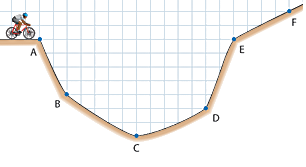
\includegraphics{Conservation_Kinetic_Potential}
    \end{center}
    Where would the bicyclist have the...
    \begin{enumerate}
        \item Highest potential energy?
        \item Lowest potential energy?
        \item Highest kinetic energy?
        \item Highest speed?
    \end{enumerate}
    Would the bicyclist's ..... be higher at A or C?
    \begin{enumerate}
        \item Kinetic energy
        \item Potential energy
        \item Total energy
    \end{enumerate}
    Suppose the bicyclist lets off the brakes and coasts down into the valley without pedaling. Even if there is no friction or air resistance to slow him down, what is the farthest point the bicyclist could reach without pedaling?
\end{exmp}
You can solve this problem by using some facts about energy.
\newline
First, use the fact that kinetic energy is energy in the form of motion, and that kinetic energy is proportional to the mass of what's moving and the square of the speed of the motion.
\begin{enumerate}
    \item That means the bicyclist has kinetic energy whenever he's moving, and that the faster he moves the more kinetic energy he has.
\end{enumerate}
Next, use the fact that potential energy is energy from the potential action of a force, and that potential energy is proportional to the strength of the force and to the distance over which it can act.
\begin{enumerate}
    \item In this case, the force is the force of gravity pulling the bicyclist down, and the distance over which it can act is his height above the bottom of the valley. (Once he reaches the bottom of the valley, gravity can't pull him any further down) That means the bicyclist's potential energy will be higher the higher he is above the valley floor.
\end{enumerate}
Finally, and most importantly, use the Principle of Conservation of Energy, which tells you that energy can neither be created nor destroyed. 
\begin{enumerate}
    \item That means as the bicyclist loses potential energy coasting downhill, he must gain an equal amount of kinetic energy (by speeding up), so that his total energy must stay constant.
    \item Similarly, when the bicyclist gains potential energy by coasting up the far side of the valley, he must lose kinetic eneryg (by slowing down), so that his total energy must stay constant.
\end{enumerate}
Now let's apply these general principles to the specific questions in this problem:
\begin{enumerate}
    \item Since his potential energy is proportional to his height above the bottom of the valley, the bicyclist would have the highest potential energy at F and the lowest at C.
    \item Since his kinetic energy increases as his potential energy decreases, the bicyclist would have the highest kinetic energy where his potential energy is the lowest, at C.
    \item Likewise, since kinetic energy is proportional to the square of speed, the speed of the bicyclist is the highest when the kinetic energy is the highest - at C. 
    \item At the entrance to the valley, the bicyclist isn't moving, so he has no kinetic energy. That means his total energy is equal to his potential energy. For the bicyclist to be able to coast up the other side of the valley to a point higher than the valley enterance (for example to point F), he'd have to have a potential energy higher than his total energy - which is impossible! \\
    Therefore, even if he loses no energy to friction with the road or air, the bicyclist can go no higher than the valley entrance without pedaling. That means the furthest point he can reach is E. 
    \item Since A is higher than C, the bicyclist's potential energy would be higher and his kinetic energy would be lower. The total energy, however, would be the same at both points.
\end{enumerate}

\section*{Calculating Solubility}
\begin{exmp}
    A geochemist in the field takes a 50mL sample of water from a rock pool lined with crystals of a certain mineral compound X. He notes the temperature of the pool, 17C, and caps the sample carefully. Back in the lab, the geochemist filters the sample and then evaporates all the water under vacuum. Crystals of X are left behind. The researcher washes, dries and weighs the crystals. They weigh 1.7g.
    \begin{enumerate}
        \item Using only the information above, can you calculate the solubility of X in water at 17C? If so, calculate it.
    \end{enumerate} 
\end{exmp}
You can solve this problem by using the fact that the solubility of a solute is equal to its concentration in a saturated solution, and a saturated solution is a solution in which \emph{no more of the solute will dissolve}.
\begin{enumerate}
    \item You \emph{know} a solution is saturated when it's in contact with extra solute that refuses to dissolve. 
    \item If there is no undissolved solute, the solution may or may not be saturated.
\end{enumerate}
In this case, you know that the solution must be saturated in X, since it's in contact with undissolved X. That means you \emph{can} calculate the solubility of X.
\newline
THe solubility of X equals the concentration of X in the saturated solution - the mass of dissolved X divided by the volume of the solution:
\begin{equation*}
    \begin{aligned}
        \frac{1.7g}{50.0mL} = 0.03400... g/mL
    \end{aligned}
\end{equation*}
There are 2 sig figs in 1.7g and 3 in 50.0 mL. So your calculated answer should have 2 sig figs.

\section*{Using the solubility of a compound to calculate $K_{sp}$}
\begin{exmp}
    The solubility of \ce{CaCO3} in water at 25C is measured to be 0.0067 g/L. Use this information to calculate $K_{sp}$ for \ce{CaCO3}.
\end{exmp}
In a saturated solution, the last bit of undissolved \ce{CaCO3} will be in equilibrium with the dissolved ions:
\begin{equation*}
    \begin{aligned}
        \ce{CaCO3(s) <=> Ca^2+(aq) + CO3^2-(aq)}
    \end{aligned}
\end{equation*}
That means the equilibrium molarities of the ions must be related to $K_{sp}$ through the $K_{sp}$ expression equation:
\begin{equation*}
    \begin{aligned}
        \ce{K_{sp} = [Ca^2+][CO3^2-]} \text{ CaCO3 doesn't appear here because it's present as a pure solid.}
    \end{aligned}
\end{equation*}
To use this equation, you first need to convert the equilibrium solubility of \ce{CaCO3} to the equilibrium molar solubility. Dividing grams per liter by the molar mass of \ce{CaCO3} will convert to moles per liter:
\begin{equation*}
    \begin{aligned}
        \frac{0.0067 g/L}{100.086 g/mol} = 6.694...*10^{-5}M
    \end{aligned}
\end{equation*}
Now use the stoichiometry in the chemical equation to find the molarities of \ce{Ca^2+} and \ce{CO3^2-}
\begin{equation*}
    \begin{aligned}
        \ce{[Ca^2+]} = 6.694*10^{-5}\\
        \ce{[CO3^2-]} = 6.694*10^{-5}
    \end{aligned}
\end{equation*}
Now you can calculate $K_{sp}$: 
\begin{equation*}
    \begin{aligned}
        K_{sp} &= (6.694*10^{-5})(6.694*10^{-5})\\
            &= 4.481*10^{-9} \\
            &= 4.5*10^{-9}
    \end{aligned}
\end{equation*}

\section*{Using $K_{sp}$ to calculate the solubility of a compound}
\begin{exmp}
    Calculate the solubility of \ce{CaF2} in water at 25C. 
\end{exmp}
In a saturated solution, the last bit of undissolved \ce{CaF2} will be in equilibrium with the dissolved ions:
\begin{equation*}
    \begin{aligned}
        \ce{CaF2 <=> CA^2+ + 2F-}
    \end{aligned}
\end{equation*}
That means you can calculate the equilibrium molarities of the ions from the $K_{sp}$ expression equation.
\begin{equation*}
    \begin{aligned}
        K_{sp} = \ce{[Ca^2+][F-]^2} \text{CaF2 doesn't appear here since its a pure solid.}
    \end{aligned}
\end{equation*}
As always when solving equilibrium composition problems, it's helpful to begin by setting up an ICE table. Let x stand for the moles per liter of \ce{CaF2} that dissolves:
\begin{center}
    \begin{tabular}{ c c c}
        X & $\ce{[Ca^2+]}$ & $\ce{[F^-]}$ \\
        I & 0 & 0  \\
        C & x & 2x \\
        E & x & 2x
    \end{tabular}
\end{center}
There's no column for \ce{CaF2}. Since it's present as the pure solid, it can't change concentration, and can't be in the reaction table.
\newline
Now substitute the expresion from the "equilibrium" line of the reaction table into the $K_{sp}$ expression:
\begin{equation*}
    \begin{aligned}
        K_{sp} &= x * (2x)^2 \\
        K_{sp} &= 4x^3 \text{Simplify.}\\
        x &= (K_{sp}/4)^{1/3} \text{Solve for x.} \\
         &= (K_{sp}/4)^{1/3} \text{Substitute Ksp from ALEKS data tab.} \\
         &= ((3.45*10^{-11})/4)^{1/3} \\
         &= 2.051*10^{-4} moles/Liter
    \end{aligned}
\end{equation*}
Multiply by molar mass to find grams per liter dissolved:
\begin{equation*}
    \begin{aligned}
        (2.051*10^{-4} \frac{mol}{L})*(78.075 \frac{g}{mol}) = 0.01601 \frac{g}{L}
    \end{aligned}
\end{equation*}

\section*{(MIDTERM) Question 6 - Order Salt Solution by Increasing pH}
Want to order everything in $K_a$, since you're given acids AND bases
\begin{enumerate}
    \item Start by ranking by the strongest acid out of the two you're given  \\
        In this case, nitrous acid > hyrocyanic acid (nitrous acid has a greater Ka than hydrocyanic acid)
    \item After this, you can do the same for your bases, in this case Aniline > Methylamine
    \item Follow this logic to sort them -
    \begin{center}
        good base pH $>$ bad base pH $>$ bad acid pH $>$ good acid pH \\
        Aliline $>$ Methylamine $>$ Hydrocyanic Acid $>$ Nitrous Acid \\
        $\ce{C6H5NH2} > \ce{CH3NH2} > \ce{HCN} > \ce{HNO2}$ \\
        $\ce{C6H5NH3Cl} > \ce{CH3NH3Br} > \ce{NaCN} > \ce{KNO2}$
    \end{center}
\end{enumerate}

\section*{(MIDTERM) Question 7a - Buffers}
You solve this problem using the HH equation:\footnote{Funnily enough using the HH equation for buffers works perfectly - professors are sussy about using HH since students will use it everywhere in really weird ways.}
\begin{equation*}
    \begin{aligned}
        pH &= \ce{pKa + log_{10}(\frac{[CH3O2COO-]}{[CH3C2COOH]})} \\
           &= (-log(1.3*10^{-5})) + log_{10}(\frac{0.1}{0.1}) \\
           &= 4.89
    \end{aligned}
\end{equation*}

\section*{(MIDTERM) Question 7b - Buffers}
\begin{equation*}
    \begin{aligned}
        pH &= \ce{pKa + log_{10}(\frac{[CH3O2COO-]}{[CH3C2COOH]})} \\
           &= (-log(1.3*10^{-5})) + log_{10}(\frac{0.12}{0.08}) \\
           &= 5.062
    \end{aligned}
\end{equation*}

\section*{Using the general properties of reaction enthalpy}
\begin{exmp}
    A chemist measures the enthalpy change $\Delta H$ during the following reaction:
    \begin{equation*}
        \begin{aligned}
            \ce{Fe_(s) + 2 HCl_(g) -> FeCl2_(s) + H2_(g)} \quad \Delta H = -157. kJ
        \end{aligned}
    \end{equation*}
    Use this information to complete the table below. Round each of your answers to the nearest kJ/mol.
    \begin{center}
        \begin{tabular}{c c}
            Reaction & $\Delta H$ \\
            \ce{3 FeCl2 + 3 H2 -> Fe + 6HCl} & ?? kJ \\
            \ce{4 Fe + 8 HCl -> 4 FeCl2 + 4 H2} & ?? kJ \\
            \ce{FeCl2 + H2 -> Fe + 2 HCl} & ?? kJ \\
        \end{tabular}
    \end{center}
\end{exmp}
You can solve this problem by using some general properties of reaction enthalpy.
In particular, if you know that the reaction enthalpy of a certain reaction is $\Delta H$, then:
\begin{enumerate}
    \item The reaction enthalpy of the reverse reaction is $-\Delta H$.
    \item The reaction enthalpy for the reaction multiplied by \emph{n} is $n\Delta H$.
    \item The reaction enthalpy for the reaction divided by \emph{n} is $\Delta H/n$. 
\end{enumerate}
Now let's apply these ideas to each equation in the table:
\begin{enumerate}
    \item The first chemical wequation is the original equation reversed \emph{and} multiplied by 3. That means its reaction enthalpy will be minus the original enthalpy multiplied by 3, which is $471.kJ$.
    \item The second chemical equation is the original equation multiplied by 4. That means its reaction enthalpy will be the original reaction enthalpy multiplied by 4, which is $-628. kJ$.
    \item The third chemical equation is the original equation reversed. That means its reaction enthalpy will be minus the original reaction enthalpy, which is $157. kJ$. 
\end{enumerate}

\section*{Calculating Specific Heat Capacity}
\begin{exmp}
    A chemist carefully measures the amount of heat needed to raise the temperature of a 0.72 kg sample of a pure substance from -9.2C to 14.3C. The experiment shows that 7.6kJ of heat are needed. What can the chemist report for the heat capacity of the substance? 
\end{exmp}
The \emph{specific heat capacity} of a substance is the amount of heat needed to raise the temperature of 1 gram of a substance by 1 kelvin. You can think of specific heat capacity as something like the "price" of a kelvin of temperature rise. It takes more heat to "buy" a kelvin when a substance demands a high "price" (has a high heat capacity) than when it demands a low "price" (has a low heat capacity).
\newline
To calculate the "price of each kelvin of temperature rise for the substance, the chemist should divide the "cost" of temperature rise (heat used per gram of substance) by the "amount" of temperature it "bought" (the kelvins the temperature rose). Here's what it looks like as an equation:
\begin{equation*}
    \begin{aligned}
        c = \frac{Q}{m*\Delta T}
    \end{aligned}
\end{equation*}
The symbol Q stands for the total heat used, m is the mass of the pure sample in the experiment, and $\Delta T$ is the temperature change.
To use this equation, the chemist will need to find the number of kelvins of temperature change:
\begin{equation*}
    \begin{aligned}
        \Delta T = 14.3C - (-9.2C) = 23.5K
    \end{aligned}
\end{equation*}
Remember that the kelvin is the exact same size as the Celsius degree. Now we can find the specific heat capacity of the pure substance:
\begin{equation*}
    \begin{aligned}
        c &= \frac{Q}{m*\Delta T} \\
        c &= \frac{7.6kJ}{(0.72kg)(23.5K)} \\
        c &= 0.45 \frac{kJ}{kg*K} \\
        c &= 0.45 \frac{J}{g*K} \\
    \end{aligned}
\end{equation*}

\section*{Calculating a molar heat of reaction from formation enthalpies}
\begin{exmp}
    Using the table of standard formation enthalpies that you'll find under the ALEKS data tab, calculate the reaction enthalpy of this reaction under standard conditions:
    \begin{equation*}
        \begin{aligned}
            \ce{2 NaOH_(s) + CaCl2_(s) -> Ca(OH)2_(s) + 2 NaCl_(s)}
        \end{aligned}
    \end{equation*}
\end{exmp}
You can solve this problem by rewriting the reaction as a sequence of standard formaation reactions, and then using Hess's Law.
First, look up the standard formation enthalpies $\Delta H^\circ_f$ of each reactant or product, using ALEKS data tab. Next, write standard formation reactions for each reactant or product:
\begin{center}
    \begin{tabular}{ c c c }
        reactant/product & $\Delta H^\circ_f$ (kJ/mol) & standard formation reaction \\
        \ce{NaOH_(s)} & -425.8 & \ce{0.5 H2 + 0.5 O2 Na -> NaOH} \\
        \ce{CaCl2_(s)} & -795.4 & \ce{Cl2 + Ca -> CaCl2} \\
        \ce{Ca(OH)2_(s)} & -985.2 & \ce{H2 + O2 + Ca -> Ca(OH)2} \\
        \ce{NaCl_(s)} & -411.2 & \ce{Na + 0.5 Cl2 -> NaCl} \\
    \end{tabular}
\end{center}
Next, imagine the reaction happening as a sequence of the formation reactions:
\begin{enumerate}
    \item In the first or "tearing down" part of the sequence, each reactant decomposes into elements in their standard states:
        \begin{equation*}
            \begin{aligned}
                &2(& \ce{NaOH -> 0.5 H2 + 0.5 O2 Na } &) & \Delta H = -2\Delta H^\circ_f [\ce{NaOH_(s)}] \\
                &+ & \ce{CaCl2 -> Cl2 + Ca }          &  &  \Delta H = -\Delta H^\circ_f [\ce{CaCl2_(s)}] \\  
                \hline
                  &&\ce{2 NaOH + CaCl -> H2 + O2 + 2 Na + Cl2 + Ca}&&
            \end{aligned}
        \end{equation*}
    \item In the second or "building up" part of the sequence, each product is formed out of elements in their standard state:
        \begin{equation*}
            \begin{aligned}
                && \ce{H2 + O2 + Ca -> Ca(OH)2} & & \Delta H = \Delta H^\circ_f [\ce{Ca(OH)2_(s)}] \\
                &+2(& ce{Na + 0.5 Cl2 -> NaCl} &)  &  \Delta H = \Delta H^\circ_f [\ce{NaCl_(s)}] \\  
                \hline
                &&\ce{H2 + O2 + 2 Na + Cl2 + Ca -> Ca(OH)2 + 2 NaCl}&&
            \end{aligned}
        \end{equation*}
    \item Combining both parts gives you the net reaction you want:
    \begin{equation*}
        \begin{aligned}
            &2(& \ce{NaOH -> 0.5 H2 + 0.5 O2 Na } &) & \Delta H = -2\Delta H^\circ_f [\ce{NaOH_(s)}] \\
            &+ & \ce{CaCl2 -> Cl2 + Ca }          &  &  \Delta H = -\Delta H^\circ_f [\ce{CaCl2_(s)}] \\ 
            &+ & \ce{H2 + O2 + Ca -> Ca(OH)2} & & \Delta H = \Delta H^\circ_f [\ce{Ca(OH)2_(s)}] \\
            &+2(& ce{Na + 0.5 Cl2 -> NaCl} &)  &  \Delta H = \Delta H^\circ_f [\ce{NaCl_(s)}] \\   
            \hline
            &&\ce{2 NaOH + CaCl -> Ca(OH)2 + 2 NaCl}&&
        \end{aligned}
    \end{equation*}
\end{enumerate}
Hess's law tells you that the net change in enthalpy for this sequence equals the sum of the change in enthalpies for each step:
\begin{equation*}
    \begin{aligned}
        \Delta H &= -2\Delta H^\circ_f [\ce{NaOH_(s)}]  -\Delta H^\circ_f [\ce{CaCl2_(s)}] +  \Delta H^\circ_f [\ce{Ca(OH)2_(s)}] + \Delta H^\circ_f [\ce{NaCl_(s)}] \\
        &= -2(-425.8 kJ) - (-795.4 kJ) + (-985.2 kJ) + 2(-411.2 kJ) \\
        \Delta H &= -160.60 kJ 
    \end{aligned}
\end{equation*}
Note that the units of $\Delta H$ are kJ, even though the units for $\Delta H^\circ_f$ are kJ/mol. That's because we are interested in the change of enthalpy when the stoichiometric coefficients are interrepreeted as the number of \emph{moles} of each reactant. Multiplying by kJ/mol gives kJ for the final units. 

\section*{Using Specific Heat Capacity to Find Heat}
\begin{exmp}
    Calculate the energy required to heat 458.0 mg of ethanol from 13.3C to 19.4C. Assume the specific heat capacity of ethanol under these conditions is 2.44 $\frac{J}{g*k}$.
\end{exmp}
When heat flows temperature may change. If flows into a substance its temperature will normally go up, and if heat flows out of a substance, its temperature will normally go down. (The temperature might not change if the substance is in the middle of melting, freezing, boiling or condensing.) 
\newline
How do you calculate how \emph{much} heat it takes to change the temperature of a substance? Whenever you need a connection between heat flow and temperature change, you should think of specific heat capacity. The specific heat capacity of a substance is the amount of heat needed to raise the temperature of a gram of a substance by kelvin. Here's its definition: 
\begin{equation*}
    \begin{aligned}
        c &= \frac{Q}{m*\Delta T} \\
    \end{aligned}
\end{equation*}
This equation would tell you how to calculate the specific heat capacity of silver if you knew how much heat had been used to raise its temperature. But you can \emph{also} re-arrange the equation, using algebra, so that you can use it to calculate the heat needed to raise the temperature when you already know the specific heat capacity:  
\begin{equation*}
    \begin{aligned}
        Q = m * c * \Delta T
    \end{aligned}
\end{equation*}
To use the re-arranged equation, you'll first need to find the temperature change of the ethanol: 
\begin{equation*}
    \begin{aligned}
        \Delta T = 19.4C - 13.3C = 6.1C = 6.1K
    \end{aligned}
\end{equation*}
Notice that a temperature difference in degrees Celsius conveniently equals the temperature difference in kelvins, since the kelvin is exactly the same size as the Celsius degree.
Now you can use the re-arranged equation to calculate the heat required to raise the temperature of the ethanol by 6.1K: 
\begin{equation*}
    \begin{aligned}
        Q &= m * c * \Delta T \\
        &= (458.0 mg)(2.44 \frac{J}{g*K})(6.1K) \\
        &= (2.44 \frac{J}{g*K})(458.0 *10^{-3}g)(6.1K) \\
        Q &= 6.8J
    \end{aligned}
\end{equation*}

\section*{Using Hess's Law to calculate net reaction enthalpy}
\begin{exmp}
    The lead-acid storage battery is the oldest rechargeable battery in existence. It was invented in 1859 by French physician Gaston Plante and still retains application today, more than 150 years later. 
    There are two reactions that take place during discharge of the lead-acid storage battery. In one step, sulfuric acid decomposes to form sulfur trioxide and water: 
    \begin{equation*}
        \begin{aligned}
            \ce{H2SO4 -> SO3 + H2O} \quad \Delta H = + 113. kJ \\
        \end{aligned}
    \end{equation*}
    In another step, lead, lead(IV) oxide, and sulfur trioxide react to form lead(II) sulfate: 
    \begin{equation*}
        \begin{aligned}
            \ce{Pb + PbO2 + 2 SO3 -> 2 PbSO4} \quad \Delta H = -775. kJ 
        \end{aligned}
    \end{equation*}
    Calculate the net change in enthalpy for the formation of \emph{one mole} of lead(II) sulfate from lead, lead(IV) oxide, and sulfuric acid from these reactions.  
\end{exmp}
You can solve this problem using the general properties of reaction enthalpy and Hess's Law. 
\begin{enumerate}
    \item Hess's Law says that the net change in enthalpy of a sequence of chemical reactions is equal to the sum of the change in enthalpies during each step of the sequence. 
\end{enumerate}
Note: it's important to keep in mind that if a particular step runs several times during the sequence, its reaction enthalpy is added once for each time it runs. 
First, notice that there's one intermediate in this sequence, sulfur trioxide (
\ce{SO3}). Also, 1 mole of sulfur trioxide is produced every time the first step runs, and 2 moles of sulfur trioxide are consumed every time the second step runs. For all the sulfur trioxide produced in the first step to be consumed in the second step, the first step must run twice for each time the second step runs. 
That means the equation of the net reaction can be found by adding up two copies of the equation in the first step and one copy of the equation in the second step, like so: 
    \begin{equation*}
        \begin{aligned}
            &2(& \ce{H2SO4 -> SO3 + H2O} &) & \\
            &+ & \ce{Pb + PbO2 + 2 SO3 -> 2 PbSO4} &  & \\  
            \hline
            &&\ce{Pb + PbO2 + 2 SO3 + 2H2SO4 -> 2 PbSO4 + 2 H2O}&&
        \end{aligned}
    \end{equation*}
Notice that the intermediate \ce{SO3} cancels out of the net reaction. 
Hess's Law tells you that you can find the net reaction enthalpy by adding up the reaction enthalpies of the steps in exactly the same way. That is, in this case, the net reaction enthalpy equals 2 times the reaction enthalpy for the first step plus the reaction enthalpy for the second step: 
\begin{equation*}
    \begin{aligned}
        & &2*113.kJ& \\
        &+&  -775.kJ&\\
        \hline
        &&-549.kJ&
    \end{aligned}
\end{equation*}
Notice that the stoichiometric coefficient of lead(II) sulfate in the equation of the net reaction is 2. That means -549. kJ is the net change in enthalpy for the formation of 2 moles of lead(II) sulfate. Since you're asked for the change in enthalpy when one mole of lead(II) sulfate is formed, so you need to divide -549. kJ by 2 to get your final answer. 

\section*{Writing a standard formation reaction}
\begin{exmp}
    Write a balanced chemical equation for the standard formation reaction of solid chromium(III) nitrate (\ce{Cr(NO3)3}). 
\end{exmp}
The standard formation reaction of a chemical compound has 1 mole of the compound as its only product, and for reactants has only elements in their standard state.
To write the equation of a standard formation reaction, follow these steps:
\begin{enumerate}
    \item Identify the elements in the compound. \\
        In this case, chromium(III) nitrate contains nitrogen, oxygen, and chromium. 
    \item Identify the standard state of each element. \\
        In this case, the standard state of nitrogen is \ce{N2_(g)}, the standard state of oxygen is \ce{O2_(g)}, and the standard state of chromium is \ce{Cr_(s)}. 
    \item Write and balance the formation reaction equation.\\
        Begin by writing all the elements in their standard state on the left-hand side of the equation, and the compound to be formed on the right-hand side: 
            \begin{equation*}
                \begin{aligned}
                    \ce{N2 + O2 + Cr -> Cr(NO3)3}
                \end{aligned}
            \end{equation*}
        Next, balance the equation: 
            \begin{equation*}
                \begin{aligned}
                    \ce{3 N2 + 9 O2 + 2 Cr -> 2 Cr(NO3)3}
                \end{aligned}
            \end{equation*}
    \item Make sure the equation has only 1 mole of product.\\
        The standard formation reaction produces one mole of the compound. If necessary, divide the formation reaction through by the stoichiometric coefficient of the product.
            \begin{equation*}
                \begin{aligned}
                    \ce{3/2 N2 + 9/2 O2 + Cr ->  Cr(NO3)3}
                \end{aligned}
            \end{equation*}
\end{enumerate}

\section*{Calculating Absolute Entropy using the Boltzmann Hypothesis}
\begin{exmp}
    An oxygen (\ce{O2}) molecule is adsorbed onto a small patch of the surface of a catalyst. It's known that the molecule is adsorbed on 1 of 25 possible sites for adsorbtion.
    \newline
    Calculate the entropy of this system.
\end{exmp}
You can answer this question using the Boltzmann definition of entropy:
\begin{equation*}
    \begin{aligned}
        S = k_B \ln W
    \end{aligned}
\end{equation*}
In the Boltzmann equation \emph{S} stands for the entropy of a system in a given thermodynamic state, and \emph{W} stands for the number of microstates of the system in that thermodynamic state. The constant out front, $k_B$, is called the Boltzmann constant.
\begin{enumerate}
    \item In this problem, the thermodynamic state of the system is described by the fact that the \ce{O2} molecule is known to be adsorbed somewhere on the patch of the surface.
    \item One \emph{microstate} of this system would be the \ce{O2} molecule adsorbed on the first site, counting from the lower left corner of the patch. Another microstate would be the molecule adsorbed on the second site, and still another microstate would be the molecule adsorbed on the third site.
\end{enumerate}
The key fact abou the microstates of a system is that it must be equally likely for the system to be in any of them, given the knowledge of the system expressed by its thermodynamic state. That's certainly true in this problem: given that we know only that the molecule is \emph{somewhere} on the surface, its equally likely for the molecule to be adsorbed on any one of the 25 sites. Therefore, there are 25 microstates consistent with the thermodynamic state.
\newline
Once you've counted \emph{W}, the nuumber of microstates, you can use the Boltzmann equation to calculate the entropy of the thermodynamic state.
\begin{equation*}
    \begin{aligned}
        S &= k_B \ln W \\
        S &= (1.38065*10^{-23} \frac{J}{K})\ln (25) \\
        S &= 4.4441 * 10{-23} \frac{J}{K}
    \end{aligned}
\end{equation*} 

\section*{Predicting qualitatively how entropy changes with temperature and volume}
\begin{exmp}
    For each system listed in the first column of the table below, decide (if possible) whether the change described in the second column will increase the entropy \emph{S} of the system, decrease \emph{S}, or leave \emph{S} unchanged.
    \newline
    \begin{tabular}{c c}
        System & Change \\
        \hline
        A few moles of helium (\ce{He}) gas. & The helium is heated from -11.0C \\
                                            & to 78.0C and is also compressed \\
                                            & from a volume of 7.0L to a volume \\
                                            &of 3.0L. \\
        A few moles of helium (\ce{He}) gas. & The helium is heated from -3.0C to \\
                                            & 54.0C while the volume is held \\
                                            & constant at 8.0L \\
        A few grams of liquid water (\ce{H2O}) & The water is cooled from 37.0C to \\
                                            &8.0C    
    \end{tabular}
\end{exmp}
You can answer this question by using the fact that entropy increases when either temperature or volume increases, as long as the other is held constant. 
\begin{enumerate}
    \item For example, if 0.10 mol of water is heated from 20C to 100C, while the volume is held constant at 1.8mL, the entropy increases. If the water is cooled back down to 20C, the entropy decreases.
    \item Similarly, if 0.10 mol of carbon dioxide (\ce{CO2}) gas expands from a volume of 1.5L to 2.0L, while the temperature is held constant at -10C, the entropy increases. If the \ce{CO2} is compressed back to 1.5L, the entropy decreases.
\end{enumerate}
Sometimes you'll be asked to predict the change in entropy of a system in which \emph{both} temperature and volume change. It's important to understand that you can only do so if both changes act in the same direction.
\begin{enumerate}
    \item For example, if the temperature of some \ce{CO2} gas is raised from 20C to 100C \emph{and} the volume increases from 1.5L to 2.0L, you can safely predict the entropy will increase. That's because both the increase in temperature and volume act to increase entropy. 
    \item However, if the temperature of some \ce{CO2} gas is \emph{lowered} from 100C to 20C while the volume is increased from 1.5L to 2.0L, you can't predict whether entropy increases, decreases, or stays the same. That's because the change in temperature and volume act in opposite directions. Figuring out whether which wins or will cancel out is difficult without detailed calculations or experimental measurement. 
\end{enumerate}
Here's a table that summarizes the possibilities:
\begin{center}
    \begin{tabular}{c | c | c | c |}
        & $\Delta T < 0$ & $\Delta T = 0$ & $\Delta T > 0$\\
        \hline
        $\Delta V < 0$ & $\Delta S < 0$ & $\Delta S < 0$ & ? \\
        \hline
        $\Delta V = 0$ & $\Delta S < 0$ & $\Delta S = 0$ & $\Delta S > 0$ \\
        \hline
        $\Delta V > 0$ & ? & $\Delta S > 0$ & $\Delta S > 0$ \\
        \hline
    \end{tabular}
\end{center}
\textbf{Note:} You'll find one more fact useful, which is that the volume of liquids and solids hardly change with temperature. 
\newline
Now let's apply these general ideas to each change listed in the table.
\begin{enumerate}
    \item In the first change listed in the table., the temperature of the system (the \ce{He} gas) increases but the volume \emph{decreases}. Since the change in temperature will act to increase entropy but the change in volume will act to decrease entropy, you can't safely predict how the entropy will change.
    \item In the second change listed in the table, the temperature of the system (the \ce{He} gas) increases while volume is held constant, meaning the entropy will increase. 
    \item In the third change listed in the table, the temperature of the system (the liquid \ce{H2O}) is decreased. Since the volume of liquids hardly change with temperature, you can assume the volume stays constant. Cooling a system with volume held constant decreases the entropy.
\end{enumerate}

\section*{Predicting qualitatively how entropy changes with mixing and seperation}
\begin{exmp}
    For each system listed in the first column of the table below, decide (if possible) whether the change described in the second column will increase the entropy \emph{S} of the system, decrease \emph{S}, or leave \emph{S} unchanged. (\emph{Note for advanced students:} you may assume ideal gas and ideal solution behavior.)
    \newline
    \begin{tabular}{c c}
        System & Change \\
        \hline
        A 0.35M solution of sucrose in      & The solution is put into a  \\
        water, and a beaker of pure water,  & semipermable bag immersed in the \\
        both at 37C.                        & water, and 50.mL of pure water \\
                                            & flows through the bag into the surose solution. \\
        \hline
        A solution made of sodium iodide & 50. mL of pure water is added to \\
        (\ce{NaI}) in water, at 73C. & the solution. \\
        \hline
        A mixture of xenon (\ce{Xe}) gas and & An additional 2L of pure \ce{N2} gas \\
        nitrogen (\ce{N2}) gas at 4atm and & is added to the mixture, with the \\
        32C. & pressure kept constant at 4 atm.   
    \end{tabular}
\end{exmp}
You can answer this question by using the fact that entropy increases when pure substances are mixed, as long as temperature and total volume stay constant.
\begin{enumerate}
    \item For example, if 10.L of nitrogen (\ce{N2}) gas at 1.0 atm and 20.0C is mixed with 10.L of oxygen (\ce{O2}) gas, also at 1.0 atm and 20.0C, the entropy increases. If the two gases are seperated by fractional condensation, the entropy decreases again.
    \item Similarly, if 100.mL of ethanol (\ce{CH3CH2OH}) is mixed with 100. mL of propanol (\ce{CH3(CH2)2OH}) at 20.C, the entropy increases. If the ethanol and propanol are seperated again by distillation, the entropy decreases again.
\end{enumerate}
Keep in mind pure substances don't have to be in the same physical state to mix. Solids and liquids can mix, for example, to form a solution. If the mixing takes place without significant release or absorbtion of heat, and without a significant change in volume, then you can be confident the entropy increases. 
\begin{enumerate}
    \item For example, if 2.0g of solid sodium chloride (\ce{NaCl}) is dissolved in 150.mL of water at 50.C, the entropy increases. If the sodium chloride is seperated from the water by distillation, the entropy decreases again.
\end{enumerate}
Also note that if mixtures are mixed with still more pure substances, the entropy will continue to increase.
\begin{enumerate}
    \item If 50.mL of pure water is added to a solution of sodium chloride in water, the entropy will increase. If 50.mL of pure water is removed from the solution by pressing some of the solution through a semipermable membrane, the entropy decreases again.
\end{enumerate}
Mixtures and solutions that form without the release or absorption of heat (so the temperature stays constant) and without any change in the total volume are called \emph{ideal solutions}. It's important to remember that it's only possible to predict that entropy changes on mixing for ideal solutions, or solutions reasonable close to ideal. \emph{It's not possible to predict the entropy change on mixing for strongly nonideal solutions without detailed calculations or experimental measurement.}
\newline
Fortunately, you're told you can assume ideal solution behavior for all systems in this question. 
\newline
Now let's apply these general ideas to each change described in the table.
\begin{enumerate}
    \item In the first change listed in the table, a mixture (sucrose and water) are mixed with a pure substance, so the entropy will increase.
    \item In the second change listed in the table, a mixture (the \ce{NaI}-water solution) is mixed with another pure substance (the pure water) so the entropy will increase.
    \item In the third change listed in the table, a pure substance (the additional \ce{N2}) is mixed with an existing mixture of pure substances, so the entropy will increase.
\end{enumerate}

\section*{Qualitatively predicting reaction entropy}
\begin{exmp}
    For each chemical reaction listed in the first column of the table below, predict the sign (positive or negative) of the reaction entropy $\Delta S_{rxn}$. If it's not possible to decide with the information given, check the "not enough information" button in the last column. \\
    Note for advanced students: Assume the temperature remains constant. Assume all gases and solutions are ideal. 
    \begin{enumerate}
        \item $\ce{CaO_(s) + CO2_(g) -> CaCO3_(s)}$
        \item $\ce{2 CH3OH_(g) + 3 O2_(g) -> 2 CO2_(g) + 4 H2O_(l)}$
        \item $\ce{N2_(g) + 3 H2_(g) -> 2 NH3_(g)}$
    \end{enumerate}

\end{exmp}
You can answer this question by using these three general rules about when entropy can be expected to increase as a result of a chemical reaction:
\begin{enumerate}
    \item Entropy rises when gases form from solids or liquids.
        \begin{enumerate}
            \item That is, when the reactants are all solids, liquids, or solutions, and at least one product is a gas, $\Delta S_{rxn}$ can be expected to be positive. That's because the entropies of gases are always much higher than the entropies of solids and liquids. 
        \end{enumerate}
    \item Entropy rises when mixtures are formed from pure substances.
        \begin{enumerate}
            \item That is, when the reactants are all pure substances, and the product is a solution or mixture of gases, $\Delta S_{rxn}$ can be expected to be positive. That's because entropy usually rises considerably when pure substances are mixed.  
        \end{enumerate}
    \item Entropy rises when the moles of gases increase.
        \begin{enumerate}
            \item That is, when the total moles of product gases is greater than the total moles of reactant gases, $\Delta S_{rxn}$ can be expected to be positive. That's because entropy rises when the total moles of atoms or molecules in a gaseous system increases. 
        \end{enumerate}
    \item Note: it's important to understand that each of these rules can be used in reverse.
        \begin{enumerate}
            \item For example, if gases are consumed in reaction, producing only liquids or solids, you can predict entropy will decrease, using Rule 1 in reverse.
            \item Similarly, if a pure substance precipitates from a solution, you can predict entropy will decrease by using Rule 2 in reverse. 
        \end{enumerate}
\end{enumerate}
Let's apply these general rules to each reaction listed in the table.
\begin{enumerate}
    \item In the first reaction, a gas (\ce{CO2}) is consumed and only liquids or solids are formed. According to Rule 1 in reverse, we expect the entropy to decrease.
    \item In the second reaction, the total number of moles of gases increases from 5 to 6. According to Rule 3 we expect the entropy to increase.
    \item In the third reaction, the total number of moles of gases decreases from 4 to 2 as a result of the reaction. According to Rule 3 in reverse we expect the entropy to decrease. 
\end{enumerate}

\section*{Calculating reaction entropy using the standard molar entropies of reactants}
\begin{exmp}
    Using the thermodynamic information in the ALEKS data tab, calculate the standard reaction entropy of the following chemical reaction: 
    \begin{equation*}
        \begin{aligned}
            \ce{N2_(g) + 3 H2_(g) -> 2NH3_(g)}
        \end{aligned}
    \end{equation*}
\end{exmp}
The information you need is the standard molar entropy $S^0$ of each reactant and each product. \\
You can find standard molar entropies by opening the ALEKS Data tab and searching for the table called Thermodynamic properties of pure substances: \\
\begin{center}
    \begin{tabular}{c c}
        reactant & $S^0$ \\
        $\ce{N2_(g)}$ & 191.6 J/(k*mol) \\
        $\ce{H2_(g)}$ & 130.7 J/(k*mol) \\
    \end{tabular}
\end{center}

\begin{center}
    \begin{tabular}{c c}
        product & $S^0$ \\
        $\ce{NH3_(g)}$ & 192.8 J/(k*mol) 
    \end{tabular}
\end{center}
To find the standard reaction entropy $\Delta S^0$ of the reaction, you must add up the total entropy of the products (because they're being produced) and subtract the total entropy of the reactants (because they're being consumed): 
\begin{equation*}
    \begin{aligned}
        \Delta S^0 = \sum_{products} n_p * S^0 - \sum_{reactants} n_r * S^0
    \end{aligned}
\end{equation*}
In this equation the $n_p$'s stand for the stoichiometric coefficients of the products and the $n_r$'s stand for the stoichiometric coefficients of the reactants.  \\
Notice that you find the total entropy contributed by each reactant by multiplying its molar entropy by the number of moles that actually take part in the reaction — that is, by the stoichiometric coefficient.\\

Now let's apply these general ideas to the specific reaction in this problem.
First, calculate the total entropy added by the creation of the products:
\begin{equation*}
    \begin{aligned}
        2mol*S^0[\ce{NH3_(g)}] \\
        2mol*(192.8 \frac{J}{mol*K}) \\
        385.6 \frac{J}{K}
    \end{aligned}
\end{equation*}
Now calculate the total entropy subtracted by the consumption of all the reactants: 
\begin{equation*}
    \begin{aligned}
        (1mol) * S^0[\ce{N2_(g)}] + (3mol) * S^0[\ce{H2_(g)}] \\
        (1mol) * (191.6 \frac{J}{mol*K}) + (3mol) * S^0[130.7 \frac{J}{mol*K}] \\
        583.7 \frac{J}{K}
    \end{aligned}
\end{equation*}
Now you can find the reaction entropy, by subtracting the total entropy destroyed by consumption of the reactants from the total entropy created by production of the products: 
\begin{equation*}
    \begin{aligned}
        \Delta S^0 = 385.6 \frac{J}{K} - 583.7 \frac{J}{K} = -198. \frac{J}{K}
    \end{aligned}
\end{equation*}

\section*{Using the conditions of spontaneity to deduce the signs of $\Delta H$ an d $\Delta S$}
\begin{exmp}
    Use the observations about each chemical reaction in the table below to determine the sign (positive or negative) of the reaction enthalpy $\Delta H$ and reaction entropy $\Delta S$.
    \begin{enumerate}
        \item  This reaction is exothermic and proceeds faster at temperatures above 130C.
        \item  This reaction is always spontaneous, but proceeds faster at temperatures below 144C.
        \item  This reaction is spontaneous except below 49C.
    \end{enumerate}
\end{exmp}
You can solve this problem using two important ideas about Gibbs free energy: 
\begin{enumerate}
    \item First, you'll need to use what the Second Law of thermodynamics tells you about reaction free energy $\Delta G$:
        \begin{center}
            \begin{tabular}{c c}
                sign of reaction free energy & what second law tells you \\
                $\Delta G < 0$ & This reaction is spontaneous \\
                $\Delta G > 0$ & The reverse of this reaction is spontaneous. \\
                $\Delta G = 0$ & Neither this reaction nor its reverse reaction is spontaneous; this system is at equilibrium.
            \end{tabular}
        \end{center}
    \item Next, you'll need to use the relationship between $\Delta G$ and reaction enthalpy $\Delta H$ and reaction entropy $\Delta S$:
        \begin{equation*}
            \begin{aligned}
                \Delta G = \Delta H - T\Delta S 
            \end{aligned}
        \end{equation*}
    \item  This equation tells you that the balance between the importance of reaction enthalpy and reaction entropy depends on the temperature T:
        \begin{enumerate}
            \item At low temperatures (T very small), $T \Delta S$ is small, which means:
                \begin{equation*}
                    \begin{aligned}
                        \Delta G \approx \Delta H 
                    \end{aligned}
                \end{equation*}
                That is, at low temperatures reactions are spontaneous ($\Delta G >  0$) only if they are exothermic ($\Delta H > 0$).
            \item Conversely, at high temperatures (T very large), $T\Delta S$ is large, which means:
                \begin{equation*}
                    \begin{aligned}
                        \Delta G \approx -T \Delta S
                    \end{aligned}
                \end{equation*}
                That is, at high temperatures reactions are spontaneous ($\Delta G < 0$) only if they increase entropy ($\Delta S > 0$).
        \end{enumerate}
    \item Putting both ideas together, we can see that, depending on the signs of $\Delta H$ and $\Delta S$, a particular reaction with a particular mix of reactants might be spontaneous at \emph{all} temperatures, spontaneous at \emph{no} temperature, or spontaneous at some temperatures, but not others. Here's a summary of how it all works out:
        \begin{center}
            \begin{tabular}{| c | c | c | c | c |}
                $\Delta H$ & $\Delta S$ & $\Delta G$ (low T) & $\Delta G$ (high T) & Description \\
                \hline
                + & + & + & - & Spontaneous at high temperatures only. \\
                + & - & + & + & Never spontaneous. \\
                - & + & - & - & Spontaneous at all temperatures. \\
                - & - & - & + & Spontaneous at low temperatures only.
            \end{tabular}
        \end{center}
    This table tells you that you can use the conditions under which a reaction is spontaneous to decide the signs of $\Delta H$ and $\Delta S$. \\
\end{enumerate}
Now let's apply these general ideas to each description in the table.
\begin{enumerate}
    \item Reaction A: The rate of reaction has nothing to do with whether it is spontaneous or not. We're told this reaction is exothermic, so $\Delta H < 0$. However, we're given no information about when this reaction is spontaneous, so there's no way to decide the sign of $\Delta S$. 
    \item Reaction B: We're told this reaction is always spontaneous, so it's described by the third line of the table above. So $\Delta H < 0$ and $\Delta S > 0$. (Note that the information about the rate of the reaction is unimportant, because the rate of a reaction has nothing to do with whether it is spontaneous or not.) 
    \item Reaction C: We're told this reaction is spontaneous only at higher temperatures (higher than 49C). That means it's described by the first line of the table above. So $\Delta H > 0$ and $\Delta S > 0$. 
\end{enumerate}

\section*{Interconverting standard Gibbs free energy and K}
\begin{exmp}
    For a certain chemical reaction, the standard Gibbs free energy of reaction is 75.1 kJ. Calculate the temperature at which the equilibrium constant $K=1.9*10^{-15}$
\end{exmp}
The key to this problem is the connection between standard Gibbs free energy of reaction $\Delta G^0$ and the equilibrium constant K:
\begin{equation*}
    \begin{aligned}
        \Delta G^0 = -RT\ln K \quad \text{T is temperature (K) and R is the gas constant (J/K)}
    \end{aligned}
\end{equation*}
You can rearrange this equation to solve for T, given $\Delta G^0$ and K:
    \begin{equation*}
        \begin{aligned}
            T &= \frac{\Delta G^0}{-R \ln K} \\
            &= \frac{75.1 kJ}{-(8.3145 J/K)\ln(7.9*10^{-15})} \\
            T &= 278.16 K \\
            T &= 5C 
        \end{aligned}
    \end{equation*}

\section*{Using the general properties of Gibbs free energy}
\begin{exmp}
    The standard reaction free energy $\Delta G^0 = -835. kJ$ for this reaction:
    \begin{equation*}
        \begin{aligned}
            \ce{2 Al_(s) + Fe2O3_(s) -> Al2O3_(s) + 2 Fe_(s)} \quad \Delta G = -835. kJ
        \end{aligned}
    \end{equation*}
    Use this information to complete the table below. Round each of your answers to the nearest kJ/mol.
    \begin{center}
        \begin{tabular}{c c}
            Reaction & $\Delta H$ \\
            \ce{Al2O3_(s) + 2 Fe_(s) -> 2 Al_(s) + Fe2O3_(s)} & ?? kJ \\
            \ce{Al_(s) + 0.5 Fe2O3_(s) -> 0.5 Al2O3_(s) + Fe_(s)} & ?? kJ \\
            \ce{2 Al2O3_(s) + 4 Fe_(s) -> 4 Al_(s) + 2 Fe2O3_(s)} & ?? kJ \\
        \end{tabular}
    \end{center}
\end{exmp}
You can solve this problem by using some general properties of reaction free energy.
In particular, if you know that the reaction free energy of a certain reaction is $\Delta G$, then:
\begin{enumerate}
    \item The reaction free energy of the reverse reaction is $-\Delta G$.
    \item The reaction free energy for the reaction multiplied by \emph{n} is $n\Delta G$.
    \item The reaction free energy for the reaction divided by \emph{n} is $\Delta G/n$. 
\end{enumerate}
Now let's apply these ideas to each equation in the table:
\begin{enumerate}
    \item The first chemical equation is the original equation reversed. That means its reaction free energy will be minus the original free energy, which is $835.kJ$.
    \item The second chemical equation is the original equation divided by 2. That means its reaction free energy will be the original reaction free energy by 2, which is $-418. kJ$.
    \item The third chemical equation is the original equation reversed \emph{and} multiplied by 2. That means its reaction free energy will be minus the original reaction free energy multiplied by 2, which is $1670. kJ$. 
\end{enumerate}

\section*{Estimating a phase transition temperature from standard thermodynamic data}
\begin{exmp}
    Using the thermodynamic information in the ALEKs data tab, calculate the boiling point of methanol (\ce{CH3OH}).
\end{exmp}
You can solve this problem using two important ideas about Gibbs free energy: \\
First, let's write a chemical equation for the equilibrium between liquid and gaseous methanol: 
\begin{equation*}
    \begin{aligned}
        \ce{CH3OH_(l) <=> CH3OH_(g)}
    \end{aligned}
\end{equation*}
And let's recall what the Second Law of thermodynamics tells you about reaction free energy $\Delta G$ of chemical equilibria: 
\begin{center}
    \begin{tabular}{c c}
        sign of reaction free energy & what second law tells you \\
        $\Delta G < 0$ & This reaction is spontaneous \\
        $\Delta G > 0$ & The reverse of this reaction is spontaneous. \\
        $\Delta G = 0$ & Neither this reaction nor its reverse reaction is spontaneous; this system is at equilibrium.
    \end{tabular}
\end{center}
What does this tell you about the equilibrium between liquid methanol and gaseous methanol? 
\begin{enumerate}
    \item Below the boiling point you know gaseous methanol spontaneously condenses—turns into liquid methanol. That is, the reverse reaction is spontaneous and $\Delta G > 0$.
    \item Above the boiling point you know liquid methanol spontaneously evaporates—turns into gaseous methanol. That is, the forward reaction is spontaneous and $\Delta G < 0$.
    \item Therefore, at exactly the boiling point, liquid and gaseous methanol are in equilibrium and $\Delta G = 0$.
\end{enumerate}
To calculate the boiling point you just need to calculate the temperature at which $\Delta G = 0$. \\
The next idea you'll need is the connection between $\Delta G$, the change in enthalpy $\Delta H$ and the change in entropy $\Delta S$:
    \begin{equation*}
        \begin{aligned}
            \Delta G = \Delta H - T\Delta S 
        \end{aligned}
    \end{equation*}
You can rearrange this equation to solve for the temperature:
    \begin{equation*}
        \begin{aligned}
            T = \frac{\Delta H - \Delta G}{\Delta S}
        \end{aligned}
    \end{equation*}
You know $\Delta G = 0$ at the boiling point. You can make a good estimate of $\Delta H$ by setting it equal to the difference between the standard formation enthalpy $\Delta H^0_f$ of liquid and gaseous methanol:
\begin{equation*}
    \begin{aligned}
        \Delta H &= \Delta H^0_f [\ce{CH3OH_(g)}] - \Delta H^0_f[\ce{CH3OH_(l)}] \\
        \Delta H &= (-201.0 kJ/mol) - (-239.2 kJ/mol) \\
        \Delta H &= 38.2 kJ/mol
    \end{aligned}
\end{equation*}
Similarly, you can get a good estimate of $\Delta S$ by setting it equal to the difference between the standard entropies $S^0$ of liquid and gaseous methanol:
\begin{equation*}
    \begin{aligned}
        \Delta S &= S^0 [\ce{CH3OH_(g)}]-S^0[\ce{CH3OH_(l)}] \\
        \Delta S &= (239.9 J/(K*mol)) - (126.8 J/(K*mol)) \\
        \Delta S &= 113.1 J/(K*mol)
    \end{aligned}
\end{equation*}
Now you can return to the equation for temperature and calculate the boiling point: 
    \begin{equation*}
        \begin{aligned}
            T &= \frac{\Delta H - \Delta G}{\Delta S} \\
            T &= \frac{38.2 \frac{kJ}{mol} - 0}{113.1 \frac{J}{K*mol}} \\
            T &= \frac{3.82*10^{-4} J/mol}{113.1 \frac{J}{K*mol}} \\
            T &= 337.75K \\
            T &= 64.60C
        \end{aligned}
    \end{equation*}

\section*{Using the Second Law to predict spontaneous change}
\begin{exmp}
    Read the descriptions of physical or chemical changes in the table below. Then decide whether the change will be spontaneous, if you can.
    \begin{enumerate}
        \item A solid precipitates from a solution, absorbing heat as it does so.
        \item A gas expands, absorbing heat from its surroundings.
        \item During an exothermic chemical reaction, two moles of gaseous reactants are turned into four moles of gaseous products.
    \end{enumerate}
\end{exmp}
The key to answering these questions is the second law of thermodynamics, which tells you that changes are spontaneous only when the entropy of the universe (system + surroundings) increases.
\begin{equation*}
    \begin{aligned}
        \Delta S_{UNIV} = \Delta S + \Delta S_{surr} > 0
    \end{aligned}
\end{equation*}
The question is: can you discover enough about $\Delta S$ and $\Delta S_{surr}$ to determine whether $\Delta S_{UNIV}$ is positive or negative? You need to look for clues in the description of the changes.  \\
The first fact to bear in mind is the Clasusis definition of entropy, which gives you a relationship between heat going into the surroundings and $\Delta S_{surr}$:
\begin{equation*}
    \begin{aligned}
        \Delta S_{surr} = \frac{Q}{T}
    \end{aligned}
\end{equation*}
So if heat is released to the surroundings $\Delta S_{surr} > 0$, but if heat is \emph{absorbed} from the surroundings $\Delta S_{surr} < 0$. \\
What about the system? These general ideas will help.
\begin{enumerate}
    \item When liquid or solid substances turn into gases, $\Delta S > 0$.
    \item When pure substances form mixture , $\Delta S > 0$. 
    \item When the number of moles of gas in a system increases, $\Delta S > 0$. 
\end{enumerate}
Finally, you'll have to consider what happens when you add $\Delta S$ and $\Delta S_{surr}$:
\begin{center}
    \begin{tabular}{| c | c | c | c |}
        $\Delta S$ & $\Delta S_{surr}$ & $\Delta S_{UNIV}$ & Spontaneous?  \\
        \hline
        + & + & + & yes  \\
        - & - & - & no \\
        + & - & ? & ? \\
        - & + & ? & ? 
    \end{tabular}
\end{center}
Now let's apply these general ideas to the changes you need to evaluate: 
\begin{enumerate}
    \item In the first change described, a mixture of two substance separates, which means $\Delta S < 0$, and heat is absorbed from the surroundings, which means $\Delta S_{surr} < 0$. The entropy of the universe decreases, which means this process is not spontaneous.
    \item In the second change described, a gas expands, which means $\Delta S > 0$, but the gas absorbs heat from its surroundings, which means $\Delta S_{surr} < 0$. Without more information, it's not possible to know how the entropy of the universe changes and therefore whether this change in spontaneous.
    \item And in the third change described, the moles of gas increase, which means $\Delta S > 0$, and heat is transferred to the surroundings, which means $\Delta S_{surr} > 0$. The entropy of the universe increases, so this process is spontaneous.
\end{enumerate}

\section*{Calculating reaction free energy under nonstandard conditions}
\begin{exmp}
    A chemist fills a reaction vessel with 0.951g silver chromate (\ce{Ag2CrO4}) solid, 0.578M silver (\ce{Ag^+}) aqueous solution, and 0.707M chromate (\ce{CrO4^2-}) aqueous solution at a temperature of 25.0C \\
    Under these conditions, calculate the reaction free energy $\Delta G$ for the following chemical reaction:
        \begin{equation*}
            \begin{aligned}
                \ce{Ag2CrO4 <=> 2 Ag^+ CrO4^2-}
            \end{aligned}
        \end{equation*}
\end{exmp}
You can calculate the standard reaction free energy $\Delta G^0$ by using the chemical equation and the standard free energy of formation $\Delta G^0_f$ of each reactant and product:
\begin{equation*}
    \begin{aligned}
        \Delta G^0 &= \sum_{products} n_p * \Delta G^0_f - \sum_{reactants} n_r * \Delta G^0_f \\
        &= (2mol) * \Delta G^0_f[\ce{Ag^+}] + (1mol) * \Delta G^0_f[\ce{CrO4^2-}] - (1mol) * \Delta G^0_f[\ce{Ag2CrO4}] \\
        &= (2mol) * (77.1 kJ/mol) + (1mol) * (-727.8 kJ/mol) - (1mol) * (-641.8 kJ/mol) \\
        \Delta G^0 &= 68.2 kJ
    \end{aligned}
\end{equation*}
Is this the reaction free energy you need? No it is not. The standard reaction free energy is measured with all reactants and products in their standard states. The pressures of all gases must be 1 atm and the molarity of all solutes must be 1M. These conditions are not true for the chemist's reaction vessel, so $\Delta G \neq \Delta G^0$. \\
However, you can always calculate $\Delta G$ from $\Delta G^0$ and the \emph{actual} pressures or molarities of reactants and products, using this equation:
    \begin{equation*}
        \begin{aligned}
            \Delta G = \Delta G^0 + RT \ln Q
        \end{aligned}
    \end{equation*}
In this equation, R stands for the gas constant in units of J/K, T stands for the absolute temperature measured in kelvins, and Q stands for the reaction quotient.\\
To use this equation, you'll need to calculate the reaction quotient for the conditions inside the chemist's reaction vessel:
    \begin{equation*}
        \begin{aligned}
            Q &= [\ce{Ag^+}]^2 [\ce{CrO4^2-}] \\
            &= (0.578)^2 (0.707) \\
            Q &= 0.23620...
        \end{aligned}
    \end{equation*}
Now you're ready to use the equation for reaction free energy. Don't forget to convert the temperature to kelvins before plugging it in.
    \begin{equation*}
        \begin{aligned}
            \Delta G &= \Delta G^0 + RT \ln Q \\
            &= (68.2 kJ) + (8.31446 J/K)(273.15 + 25)\ln(0.23620) \\
            &= (68.2 kJ) + (-3577.323 J) \\
            &= (68.2 kJ) + (-3.577323 J) \\
            \Delta G &= 64.6 kJ 
        \end{aligned}
    \end{equation*}

%-------------------------------------------------------------------------------


\newpage
\section*{Scratch Work}

\begin{equation*}
    \begin{aligned}
        &0.521 = \frac{(4+2x)(x)}{(1.2-x)(2.4-x)} \\
        &0.521 * (1.2-x)(2.4-x) = 4x+ 2x^2 \\ 
        &K * (I_a - x)(I_b - x) = (I_c + 2x)(I_d + x)\\
        &K * (I_a* I_b - (I_a + I_b)x + x^2) = I_c* I_d - 2(I_c + I_d)x + 2x^2 \\
        &K(I_a* I_b) - K(I_a + I_b)x + Kx^2 = (I_c* I_d) - 2(I_c + I_d)x + 2x^2 \\
        &K(I_a* I_b) - (I_c* I_d) + K(I_a + I_b)x - 2(I_c + I_d)x + Kx^2 - 2x^2 = 0 \\
        &0.521(1.2*2.4) - (4*0) + 0.521(1.2 + 2.4)x - 2(4+0)x + 0.521x^2 - 2x^2 = 0 \\
        &1.50048 + 1.87560x - 8x - (0.521-8)x^2 = 0
    \end{aligned}
\end{equation*}

\begin{tabular}{c|c@{}c@{}c@{}c@{}c@{}c@{}c}
    \hline
    X   & $[HBrO]$ & ${}+{}$ & $[H_2O]$ & ${}\leftrightharpoons{}$ & $[BrO^-]$ & ${}+{}$ & $[H_3O^+]$ \\
    \hline
    I   &  0.88    &&     &&  0   && 0  \\
    C   &   -x   &&     &&  x   &&  x \\
    E   &   0.88-x   &&     &&   x  && x  \\      
\end{tabular}

\begin{equation*}
    \begin{aligned}
        K_a = \frac{x^2}{0.88-x} \\
        2.3*10^-9 * 0.88 = x^2 \\
        x = 4.49889*10^{-5} \\
        pH = -log_{10}(x)     
    \end{aligned}
\end{equation*}

For any weak acid with Ka and inital concentration M assuming small x approximation:
\begin{equation}
    pH = - log_{10}(K_a*M)
\end{equation}

\begin{tabular}{c|c@{}c@{}c@{}c@{}c@{}c@{}c}
    \hline
    X   & $[HA]$ & ${}+{}$ & $[H_2O]$ & *${}\leftrightharpoons{}$ & $[H_3O^+]$ & ${}+{}$ & $[A^-]$ \\
    \hline
    I   &  1.9    &&     &&  0   && 0  \\
    C   &   -x   &&     &&  x   &&  x \\
    E   &   1.9-x   &&     &&   x  && x  \\      
\end{tabular}

\begin{equation*}
    \begin{aligned}
        K_a &= \frac{[H_3O^+][A^-]}{[HA]} \\
        K_a &= \frac{x^2}{1.9-x} \\
        K_a &= \frac{x^2}{1.9} \\
        6.0*10^{-6}*(1.9) &= x^2 \\
        x &= \sqrt{6.0*10^{-6}*(1.9)} \\
        [H^+] &= 0.00337... \\
        pH &= -log_{10}\left(\sqrt{6.0*10^{-6}*(1.9)}\right) \\
        pH &= 2.47154757433
    \end{aligned}
\end{equation*}

If K = 5, then the ratio of products to reactants will be 5 - I'm assuming that we can ignore the number of atoms in each molecule so we can make it easier to determine whether the solution is in equilibrium.
\begin{equation*}
    \begin{aligned}
        \text{Product} = 8 \\
        \text{Reactant} = 2 \\
        \frac{P}{R} = \frac{8}{2} = 4 \\
    \end{aligned}
\end{equation*}
Thus the solution isn't in equilibrium.

...For K = 11
\begin{equation*}
    \begin{aligned}
        \text{Product} = 11 \\
        \text{Reactant} = 1 \\
        \frac{P}{R} = \frac{11}{1} = 11 \\
    \end{aligned}
\end{equation*}

Finding pOH - done by subtracting pH from 14:
\begin{equation*}
    \begin{aligned}
        pOH = 14 - pH
    \end{aligned}
\end{equation*} 

Finding \% evaporated since isolated:
\begin{enumerate}
    \item Parsons Concentration is 69 $\frac{g}{L}$
    \item Regular Concentration is 2.2 $\frac{g}{L}$
    \item Setting up equation:
    \begin{equation*}
        \begin{aligned}
            C_0 = C_i = 2.2 \frac{g}{L} \\
        \end{aligned}
    \end{equation*}
    \item Presently, 
    \begin{equation*}
        \begin{aligned}
            xC_0 = 69 \\
            C_0 = 2.2 \\
            x(2.2) = 69 \\
            x = \frac{69}{2.2}  = 31.36 \text{times more salty}\\
            \frac{100}{31.36} = 2.75\% 
            \text{Percent Evaporated} = 100 - 2.75 = 97.25
        \end{aligned}
    \end{equation*}
\end{enumerate}

Finding Equilibrium Constant for Reaction: \\
\ce{H2C2O4 -> 2H^+ + C2O4^2-}
K = \ce{\frac{[H]^2[C2O4]}{[H2C2O4]}}

\begin{equation*}
    \begin{aligned}
        \ce{2NH3_(g) <=> N2_(g) + 3H2_(g)}
    \end{aligned}
\end{equation*}

Finding inital concentration for ammonia:
\begin{equation*}
    \begin{aligned}
        &M = \frac{[NH_3]}{V} = \frac{2.2}{0.2} \\
        &M = 11M
    \end{aligned}
\end{equation*}

\begin{tabular}{c|c@{}c@{}c@{}c@{}c}
    \hline
    X   &   $[2NH_3]$ & ${}\leftrightharpoons{}$ & $[N_2]$ & ${}+{}$ & $[3H_2]$\\
    \hline
    I   & 11          &&   0                           &&  0       \\
    C   & -2x         &&   x                           &&  3x      \\
    E   & 11 - 2x     &&   x                           &&  3x      \\
    \hline
\end{tabular}

Creating $K_c$:
\begin{equation*}
    \begin{aligned}
        K_c &= \frac{[N_2][H_2]^3}{[NH_3]^2} \\
            &= \frac{[x][3x]^3}{[11-2x]^2} \\
    \end{aligned}
\end{equation*}

Plugging in $[H_2] = 1.7/0.2 = 8.5M$ and applying small-x approximation:
\begin{equation*}
    \begin{aligned}
        K_c &= \frac{[N_2][H_2]^3}{[NH_3]^2} \\
            &= \frac{[x][8.5]^3}{[11]^2} \\
    \end{aligned}
\end{equation*}

\begin{equation*}
    \begin{aligned}
        K = \ce{\frac{[H_2] [Cl_2]}{[HCl^2]}}
    \end{aligned}
\end{equation*}
Finding M/L for HCl:
\begin{equation*}
    \begin{aligned}
        M = \frac{0.39mol}{17L} = 2.3*10^{-2}M
    \end{aligned}
\end{equation*}

Important for finding K - since HCl is a strong acid, there will be no HCl at equilibrium ideally. And since we have 2M HCl for H2 and Cl2 respectively, the final K will be $\left(2.3*10^-2\right)^2$

\begin{tabular}{c|c@{}c@{}c@{}c@{}c}
    \hline
    X   &   $[2HCl]$ & ${}\leftrightharpoons{}$ & $[H_2]$ & ${}+{}$ & $[Cl_2]$\\
    \hline
    I   &  0.023     &&   0                            &&  0       \\
    C   &       -2x      &&   x                           &&  x      \\
    E   &   0.023 - 2x     &&   x                           &&  x      \\
    \hline
\end{tabular}

\begin{equation*}
    \begin{aligned}
        K &= \ce{\frac{[H_2] [Cl_2]}{[HCl^2]}} \\
        K &= \frac{x*x}{0.023 - 2x} \\
        (0.023 - 2x)K &= x^2 \\
        0.023K - 
    \end{aligned}
\end{equation*}



Ammonia decomposition:
\begin{equation*}
    \begin{aligned}
        \ce{2NH3 -> 3H2 + N2}
    \end{aligned}
\end{equation*}
if we have 4.5 atm of ammonia gas, and have 1.4 atm of nitrogen gas in a 5L 

Create ICE Table \\
\begin{tabular}{c|c@{}c@{}c@{}c@{}c}
    \hline
    X   &   $[2NH_3]$ & ${}\leftrightharpoons{}$ & $[N_2]$ & ${}+{}$ & $[3H_2]$\\
    \hline
    I   &       4.5     &&   0                            &&  0       \\
    C   &       -2x      &&   x                           &&  3x      \\
    E   &   4.5 - 2x     &&   x                           &&  3x      \\
    \hline
\end{tabular}
\begin{equation*}
    \begin{aligned}
        K_P &= \frac{[N_2] [H_2]^3}{[NH_3]^2} \\
            &= \frac{x(3x)}{(4.5-2x)^3} \\
            &= \frac{1.4(3*1.4)}{(4.5-2*1.4)^3} 
    \end{aligned}
\end{equation*}

Sulfur dioxide and oxygen gas react too make sulfur trioxide reaction:
\begin{equation*}
    \begin{aligned}
        \ce{2SO2 + O2 -> 2SO3}
    \end{aligned}
\end{equation*}

Create ICE Table \\
\begin{tabular}{c|c@{}c@{}c@{}c@{}c}
    \hline
    X   &   $[2SO_2]$ & ${}+{}$ & $[O_2]$ & ${}\leftrightharpoons{}$ & $[2SO_3]$ \\
    \hline
    I   &       0.3066       &&   0.4133        &&  0       \\
    C   &       -2x      &&   -x        &&  2x      \\
    E   &       0.3066 - 2x     &&   0.4133 - x        &&  2x      \\
    \hline
\end{tabular}

\begin{equation*}
    \begin{aligned}
        K_b = \ce{\frac{[(CH3)2NH^+][OH-]}{(CH3)2NH}}
    \end{aligned}
\end{equation*}

\begin{equation*}
    \begin{aligned}
        K_b = \ce{\frac{[(CH3)3NH+][OH-]}{(CH3)3N}}
    \end{aligned}
\end{equation*}

Original
\begin{equation*}
    \begin{aligned}
        O = 4 \\
        d = 6 
    \end{aligned}
\end{equation*}
Box C
\begin{equation*}
    \begin{aligned}
        O = 4 \\
        d = 6 
    \end{aligned}
\end{equation*}

Box E
\begin{equation*}
    \begin{aligned}
        O = 5 \\
        d = 5 
    \end{aligned}
\end{equation*}

\subsection*{CHEM Lab Exp. 3 - Buffers}
\subsubsection*{Introduction} 
To prepare, determine, and compare the buffering capacity of various solutions.
\subsubsection*{Method}
Part A - Solution Prep:
\begin{enumerate}
    \item Clean glassware with soap and brushes in lab. Rinse and dry beakers, shaking excess water from clean test tubes.
    \item Label test tubes 1-6.
\end{enumerate}

\end{document}